\uc{Creazione conversazione}{conv}
\begin{itemize}
    \item \textbf{Attori coinvolti}: Installatore;
    \item \textbf{Descrizione}: L’installatore desidera interrogare il \textit{sistema}\textsubscript{G}, quindi crea una nuova conversazione per richiedere le informazioni a lui necessarie;
    \item \textbf{Precondizioni}: L’installatore ha accesso all’\textit{interfaccia web}\textsubscript{G} del \textit{sistema}\textsubscript{G};
    \item \textbf{Postcondizioni}: Il \textit{sistema}\textsubscript{G} crea una nuova conversazione a cui puó accedere l’installatore, dove potrà porre liberamente domande al \textit{sistema}\textsubscript{G};
    \item \textbf{Scenario principale}:
    \begin{enumerate}
        \item L’installatore accede all’\textit{interfaccia web}\textsubscript{G} di Vimar GENIALE;
        \item Richiede la creazione di una nuova conversazione;
        \item Il \textit{sistema}\textsubscript{G} esegue la creazione della nuova conversazione;
        \item  L’installatore accede alla nuova conversazione.
    \end{enumerate}
    \item \textbf{Estensioni}: UC2 - Raggiungimento limite di conversazioni.
\end{itemize}
\begin{figure}[H]
\centering
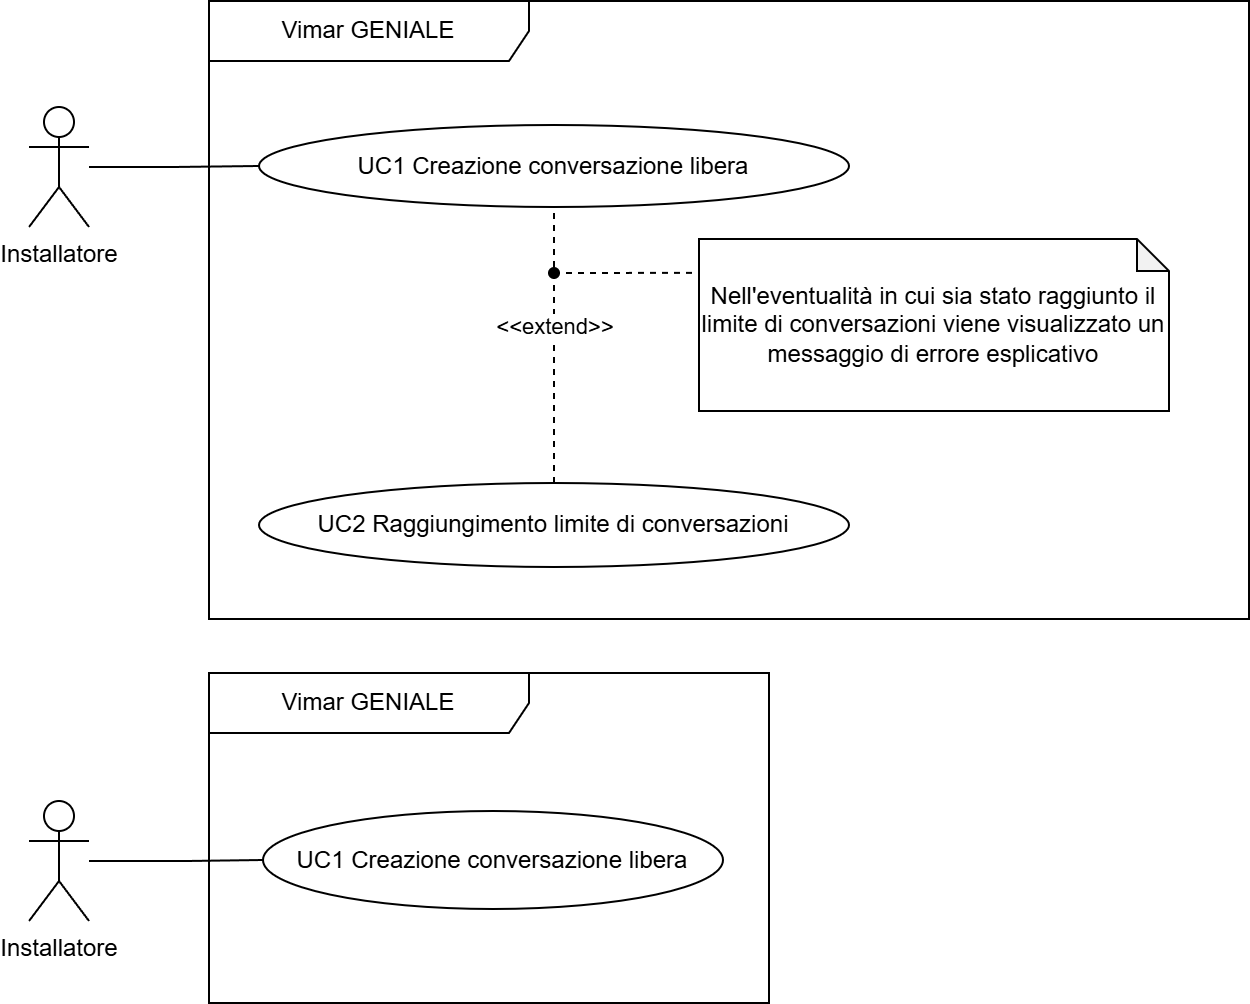
\includegraphics[width=1\textwidth]{contents/casi_duso/png/UC1.png}
\caption{UC1 - Creazione conversazione}
% \label{fig:UC1a}
\end{figure}

\subuc{Creazione \textit{conversazione libera}\textsubscript{G}}{conv_libera}
\begin{itemize}
    \item \textbf{Attori coinvolti}: Installatore;
    \item \textbf{Descrizione}: L’installatore desidera interrogare il \textit{sistema}\textsubscript{G}, quindi crea una nuova \textit{conversazione libera}\textsubscript{G} per richiedere le informazioni a lui necessarie tramite domande poste in linguaggio naturale;
    \item \textbf{Precondizioni}: L’installatore ha accesso all’\textit{interfaccia web}\textsubscript{G} del \textit{sistema}\textsubscript{G};
    \item \textbf{Postcondizioni}: Il \textit{sistema}\textsubscript{G} crea una nuova \textit{conversazione libera}\textsubscript{G} a cui puó accedere l’installatore, dove potrà porre liberamente domande in linguaggio naturale al \textit{sistema}\textsubscript{G};
    \item \textbf{Scenario principale}:
    \begin{enumerate}
        \item L’installatore accede all’\textit{interfaccia web}\textsubscript{G} di Vimar GENIALE;
        \item Richiede la creazione di una nuova conversazione in modalità libera;
        \item Il \textit{sistema}\textsubscript{G} esegue la creazione della nuova conversazione nella modalità desiderata dall’utente;
        \item  L’installatore accede alla nuova conversazione.
    \end{enumerate}
    \item \textbf{Generalizzazioni}: UC1 - Creazione conversazione.
\end{itemize}

\subuc{Creazione \textit{conversazione giudata}\textsubscript{G}}{conv_guidata}
\begin{itemize}
    \item \textbf{Attori coinvolti}: Installatore;
    \item \textbf{Descrizione}: L’installatore desidera interrogare il \textit{sistema}\textsubscript{G}, quindi crea una nuova \textit{conversazione guidata}\textsubscript{G} per richiedere le informazioni a lui necessarie tramite un prompt costruito con l’aiuto di un menù di suggerimenti;
    \item \textbf{Precondizioni}: L’installatore ha accesso all’\textit{interfaccia web}\textsubscript{G} del \textit{sistema}\textsubscript{G};
    \item \textbf{Postcondizioni}: Il \textit{sistema}\textsubscript{G} crea una nuova \textit{conversazione guidata}\textsubscript{G} a cui puó accedere l’installatore, dove potrà porre liberamente domande, realizzate con l'aiuto di menù di suggerimenti, al \textit{sistema}\textsubscript{G};
    \item \textbf{Scenario principale}:
    \begin{enumerate}
        \item L’installatore accede all’\textit{interfaccia web}\textsubscript{G} di Vimar GENIALE;
        \item Richiede la creazione di una nuova conversazione in modalità guidata;
        \item Il \textit{sistema}\textsubscript{G} esegue la creazione della nuova conversazione nella modalità desiderata dall’utente;
        \item  L’installatore accede alla nuova conversazione.
    \end{enumerate}
    \item \textbf{Generalizzazioni}: UC1 - Creazione conversazione.
\end{itemize}

\uc{Raggiungimento limite di conversazioni}{limite_conv}
\begin{itemize}
    \item \textbf{Attori coinvolti}: Installatore;
    \item \textbf{Descrizione}: L’installatore desidera interrogare il \textit{sistema}\textsubscript{G}, ma quando prova a creare una nuova conversazione per richiedere le informazioni a lui necessarie, supera il limite massimo di conversazioni supportate;
    \item \textbf{Precondizioni}: 
    \begin{itemize}
        \item L’installatore ha accesso all’\textit{interfaccia web}\textsubscript{G} del \textit{sistema}\textsubscript{G};
        \item Il numero di conversazioni memorizzate nel \textit{sistema}\textsubscript{G} supera il limite massimo supportato.
    \end{itemize}
    \item \textbf{Postcondizioni}:  Il \textit{sistema}\textsubscript{G} restituisce una risposta che indica il motivo per cui si è verificato l’errore;
    \item \textbf{Scenario principale}:
    \begin{enumerate}
        \item L’installatore accede all’\textit{interfaccia web}\textsubscript{G} di Vimar GENIALE;
        \item Richiede la creazione di una nuova conversazione, nonostante siano già esistenti un numero di conversazioni che raggiunge il limite;
        \item Il \textit{sistema}\textsubscript{G} elabora la richiesta e fornisce una risposta che spiega la causa dell'errore riscontrato;
        \item L’installatore visualizza le informazioni sull’errore che si è verificato.
    \end{enumerate}
\end{itemize}



\uc{Visualizzazione dettagli della singola conversazione}{visual_dettagli_conv}
\begin{itemize}
    \item \textbf{Attori coinvolti}: Installatore;
    \item \textbf{Descrizione}: L'installatore vuole visualizzare la conversazione da lui selezionata;
    \item \textbf{Precondizioni}: 
    \begin{itemize}
        \item L’installatore ha accesso all’\textit{interfaccia web}\textsubscript{G} del \textit{sistema}\textsubscript{G};
        \item L’installatore ha accesso ad una conversazione memorizzabile nel \textit{sistema}\textsubscript{G}.
    \end{itemize}
    \item \textbf{Postcondizioni}: L'installatore visualizza la conversazione da lui selezionata;
    \item \textbf{Scenario principale}:
    \begin{enumerate}
        \item L’installatore ha accesso all’\textit{interfaccia web}\textsubscript{G} del \textit{sistema}\textsubscript{G};
        \item L’installatore ha accesso ad una conversazione memorizzabile (o memorizzata) nel \textit{sistema}\textsubscript{G};
        \item L'installatore visualizza la conversazione selezionata.
    \end{enumerate}
    \item \textbf{Inclusioni}: 
    \begin{itemize}
        \item UC3.3 - Visualizzazione campo per inserimento prompt;
        \item UC3.4 - Visualizzazione storico dei messaggi.
    \end{itemize}
\end{itemize}

\subuc{Visualizzazione conversazione libera}{visual_conv_libera}
\begin{itemize}
    \item \textbf{Attori coinvolti}: Installatore;
    \item \textbf{Descrizione}: L'installatore vuole visualizzare la conversazione, creata in modalità libera, da lui selezionata;
    \item \textbf{Precondizioni}: 
    \begin{itemize}
        \item L’installatore ha accesso all’\textit{interfaccia web}\textsubscript{G} del \textit{sistema}\textsubscript{G};
        \item L’installatore ha accesso ad una conversazione libera memorizzabile nel \textit{sistema}\textsubscript{G}.
    \end{itemize}
    \item \textbf{Postcondizioni}: L'installatore visualizza la conversazione libera da lui selezionata;
    \item \textbf{Scenario principale}:
    \begin{enumerate}
        \item L’installatore ha accesso all’\textit{interfaccia web}\textsubscript{G} del \textit{sistema}\textsubscript{G};
        \item L’installatore ha accesso ad una conversazione libera memorizzabile (o memorizzata) nel \textit{sistema}\textsubscript{G};
        \item L'installatore visualizza la conversazione libera selezionata.
    \end{enumerate}
    \item \textbf{Inclusioni}: UC3.1.1 - Visualizzazione suggerimento sulla domanda successiva.
\end{itemize}
\begin{figure}[H]
\centering
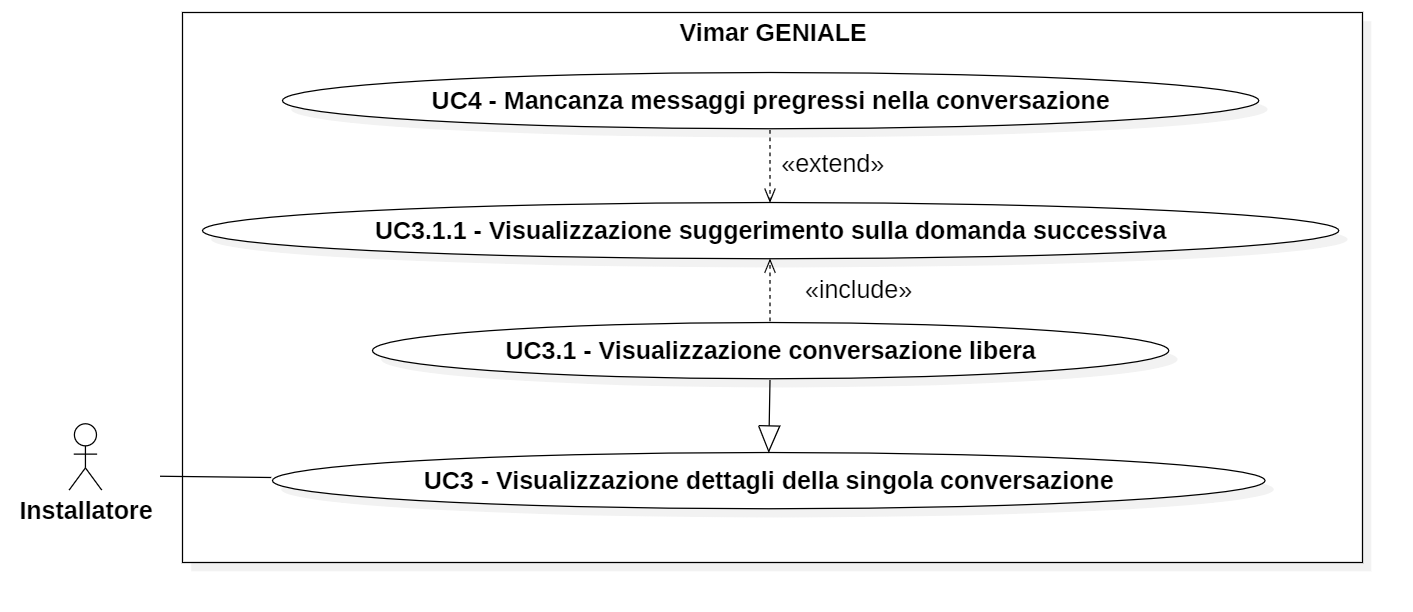
\includegraphics[width=1\textwidth]{contents/casi_duso/png/UC3.1.png}
\caption{UC3.1 - Visualizzazione conversazione libera}
% \label{fig:UC1a}
\end{figure}

\subsubuc{Visualizzazione suggerimento sulla domanda successiva}{visual_conv}
\begin{itemize}
    \item \textbf{Attori coinvolti}: Installatore;
    \item \textbf{Descrizione}: L'installatore, dopo aver posto una domanda al \textit{sistema}\textsubscript{G}, vuole visualizzare un suggerimento per la prossima domanda da porre in quella conversazione;
    \item \textbf{Precondizioni}: 
    \begin{itemize}
        \item L’installatore ha accesso all’\textit{interfaccia web}\textsubscript{G} del \textit{sistema}\textsubscript{G};
        \item L’installatore ha accesso ad una conversazione memorizzabile nel \textit{sistema}\textsubscript{G};
        \item L'installatore ha posto una domanda al sistema;
        \item Il \textit{sistema}\textsubscript{G} ha fornito una risposta ad un’interrogazione da parte dell’installatore.
    \end{itemize}
    \item \textbf{Postcondizioni}: L'installatore visualizza un suggerimento per la prossima domanda da porre al \textit{sistema}\textsubscript{G} in quella conversazione;
    \item \textbf{Scenario principale}:
    \begin{enumerate}
        \item L’installatore ha accesso all’\textit{interfaccia web}\textsubscript{G} del \textit{sistema}\textsubscript{G};
        \item L’installatore ha accesso ad una conversazione memorizzabile (o memorizzata) nel \textit{sistema}\textsubscript{G};
        \item L'installatore visualizza la conversazione selezionata;
        \item L'installatore visualizza un suggerimento per la prossima domanda da porre.
    \end{enumerate}
    \item \textbf{Estensioni}: UC4 - Mancanza messaggi pregressi nella conversazione.
\end{itemize}

\subuc{Visualizzazione conversazione guidata}{visual_conv_guidata}
\begin{itemize}
    \item \textbf{Attori coinvolti}: Installatore;
    \item \textbf{Descrizione}: L'installatore vuole visualizzare la conversazione, creata in modalità guidata, da lui selezionata;
    \item \textbf{Precondizioni}: 
    \begin{itemize}
        \item L’installatore ha accesso all’\textit{interfaccia web}\textsubscript{G} del \textit{sistema}\textsubscript{G};
        \item L’installatore ha accesso ad una conversazione guidata memorizzabile nel \textit{sistema}\textsubscript{G}.
    \end{itemize}
    \item \textbf{Postcondizioni}: L'installatore visualizza la conversazione guidata da lui selezionata;
    \item \textbf{Scenario principale}:
    \begin{enumerate}
        \item L’installatore ha accesso all’\textit{interfaccia web}\textsubscript{G} del \textit{sistema}\textsubscript{G};
        \item L’installatore ha accesso ad una conversazione guidata memorizzabile (o memorizzata) nel \textit{sistema}\textsubscript{G};
        \item L'installatore visualizza la conversazione guidata selezionata.
    \end{enumerate}
    \item \textbf{Inclusioni}: UC3.2.1 - Visualizzazione lista menù di suggerimenti.
\end{itemize}
\begin{figure}[H]
\centering
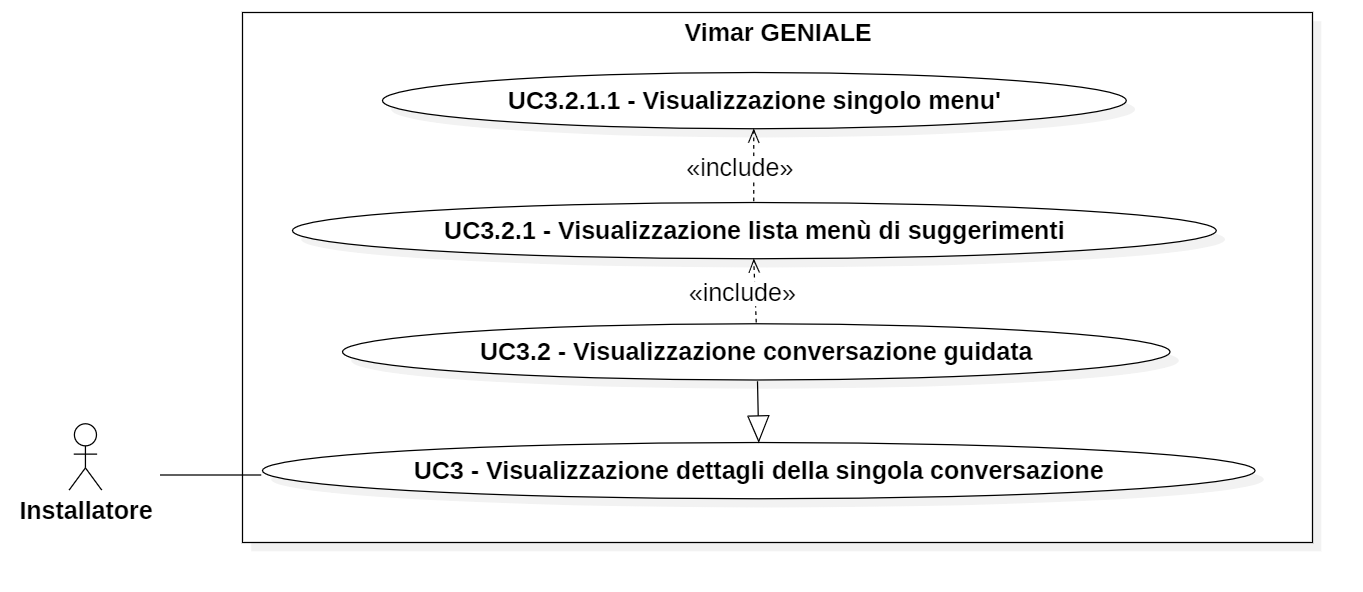
\includegraphics[width=1\textwidth]{contents/casi_duso/png/UC3.2.png}
\caption{UC3.2 - Visualizzazione conversazione guidata}
% \label{fig:UC1a}
\end{figure}

\subsubuc{Visualizzazione lista menù di suggerimenti}{visual_list_menu}
\begin{itemize}
    \item \textbf{Attori coinvolti}: Installatore;
    \item \textbf{Descrizione}: L'installatore vuole visualizzare la lista dei menù di suggerimenti per la costruzione del prompt da utilizzare nelle richieste di informazioni con conversazioni guidate;
    \item \textbf{Precondizioni}: 
    \begin{itemize}
        \item L’installatore ha accesso all’\textit{interfaccia web}\textsubscript{G} del \textit{sistema}\textsubscript{G};
        \item L’installatore ha accesso ad una conversazione guidata memorizzabile nel \textit{sistema}\textsubscript{G}.
    \end{itemize}
    \item \textbf{Postcondizioni}: L'installatore visualizza la lista dei menù di suggerimenti utilizzabili nelle conversazioni guidate;
    \item \textbf{Scenario principale}:
    \begin{enumerate}
        \item L’installatore ha accesso all’\textit{interfaccia web}\textsubscript{G} del \textit{sistema}\textsubscript{G};
        \item L’installatore ha accesso ad una conversazione guidata memorizzabile (o memorizzata) nel \textit{sistema}\textsubscript{G};
        \item L'installatore visualizza la conversazione guidata selezionata;
        \item L'installatore visualizza la lista dei menù di suggerimenti per il prompt.
    \end{enumerate}
    \item \textbf{Inclusioni}: UC3.2.1.1 - Visualizzazione singolo menù.
\end{itemize}

\subsubsubuc{Visualizzazione singolo menù}{visual_menu}
\begin{itemize}
    \item \textbf{Attori coinvolti}: Installatore;
    \item \textbf{Descrizione}: L'installatore vuole visualizzare un singolo menù appartenente alla lista dei menù di suggerimenti per la costruzione del prompt da utilizzare nelle richieste di informazioni con conversazioni guidate;
    \item \textbf{Precondizioni}: 
    \begin{itemize}
        \item L’installatore ha accesso all’\textit{interfaccia web}\textsubscript{G} del \textit{sistema}\textsubscript{G};
        \item L’installatore ha accesso ad una conversazione guidata memorizzabile nel \textit{sistema}\textsubscript{G}.
    \end{itemize}
    \item \textbf{Postcondizioni}: L'installatore visualizza un singolo menù di suggerimenti utilizzabili nelle conversazioni guidate;
    \item \textbf{Scenario principale}:
    \begin{enumerate}
        \item L’installatore ha accesso all’\textit{interfaccia web}\textsubscript{G} del \textit{sistema}\textsubscript{G};
        \item L’installatore ha accesso ad una conversazione guidata memorizzabile (o memorizzata) nel \textit{sistema}\textsubscript{G};
        \item L'installatore visualizza la conversazione guidata selezionata;
        \item L'installatore visualizza la lista dei menù di suggerimenti per il prompt;
        \item L'installatore visualizza un singolo menù di suggerimenti per il prompt.
    \end{enumerate}
\end{itemize}

\subuc{Visualizzazione campo per inserimento prompt}{visual_prompt}
\begin{itemize}
    \item \textbf{Attori coinvolti}: Installatore;
    \item \textbf{Descrizione}: L'installatore vuole visualizzare il campo in cui inserire la domanda che desidere porre al sistema;
    \item \textbf{Precondizioni}: 
    \begin{itemize}
        \item L’installatore ha accesso all’\textit{interfaccia web}\textsubscript{G} del \textit{sistema}\textsubscript{G};
        \item L’installatore ha accesso ad una conversazione memorizzabile nel \textit{sistema}\textsubscript{G}.
    \end{itemize}
    \item \textbf{Postcondizioni}: L'installatore visualizza il campo destinato all'inserimento del prompt della domanda;
    \item \textbf{Scenario principale}:
    \begin{enumerate}
        \item L’installatore ha accesso all’\textit{interfaccia web}\textsubscript{G} del \textit{sistema}\textsubscript{G};
        \item L’installatore ha accesso ad una conversazione memorizzabile (o memorizzata) nel \textit{sistema}\textsubscript{G};
        \item L'installatore visualizza la conversazione selezionata;
        \item L'installatore visualizza il campo destinato all'inserimento del prompt della domanda.
    \end{enumerate}
\end{itemize}
\begin{figure}[H]
\centering
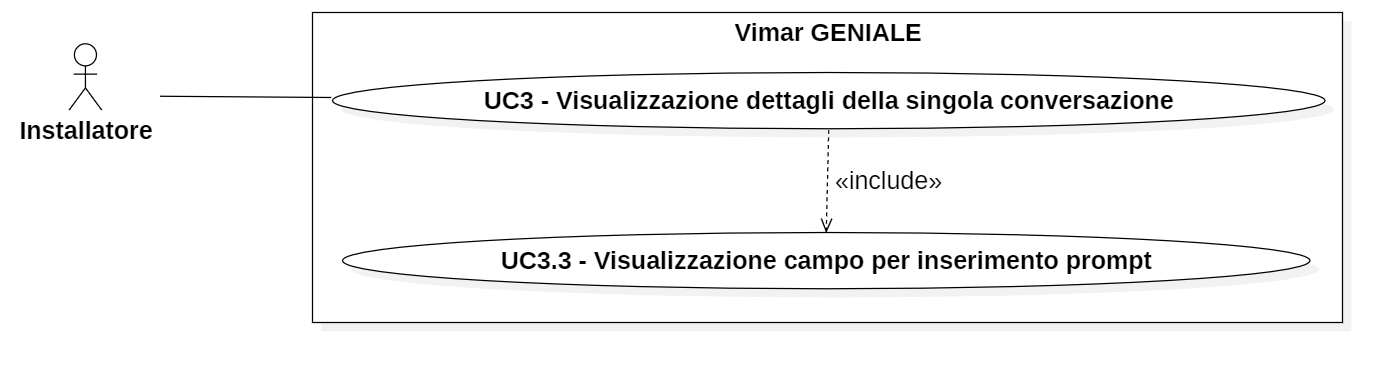
\includegraphics[width=1\textwidth]{contents/casi_duso/png/UC3.3.png}
\caption{UC3.3 - Visualizzazione campo per inserimento prompt}
% \label{fig:UC1a}
\end{figure}

\subuc{Visualizzazione storico dei messaggi}{visual_storico}
\begin{itemize}
    \item \textbf{Attori coinvolti}: Installatore;
    \item \textbf{Descrizione}: L'installatore vuole visualizzare lo storico dei messaggi della conversazione selezionata per riesaminare le risposte fornite in precedenza;
    \item \textbf{Precondizioni}: 
    \begin{itemize}
        \item L’installatore ha accesso all’\textit{interfaccia web}\textsubscript{G} del \textit{sistema}\textsubscript{G};
        \item L’installatore ha accesso ad una conversazione memorizzabile nel \textit{sistema}\textsubscript{G};
        \item L'installatore ha posto una domanda al \textit{sistema}\textsubscript{G}.
    \end{itemize}
    \item \textbf{Postcondizioni}: L'installatore visualizza lo storico dei messaggi della conversazione da lui selezionata;
    \item \textbf{Scenario principale}:
    \begin{enumerate}
        \item L’installatore ha accesso all’\textit{interfaccia web}\textsubscript{G} del \textit{sistema}\textsubscript{G};
        \item L’installatore ha accesso ad una conversazione memorizzabile (o memorizzata) nel \textit{sistema}\textsubscript{G};
        \item L'installatore visualizza la conversazione selezionata;
        \item L'installatore visualizza lo storico dei messaggi della conversazione selezionata.
    \end{enumerate}
    \item \textbf{Inclusioni}: UC3.4.1 - Visualizzazione singolo messaggio;
    \item \textbf{Estensioni}: UC4 - Mancanza messaggi pregressi nella conversazione.
\end{itemize}
\begin{figure}[H]
\centering
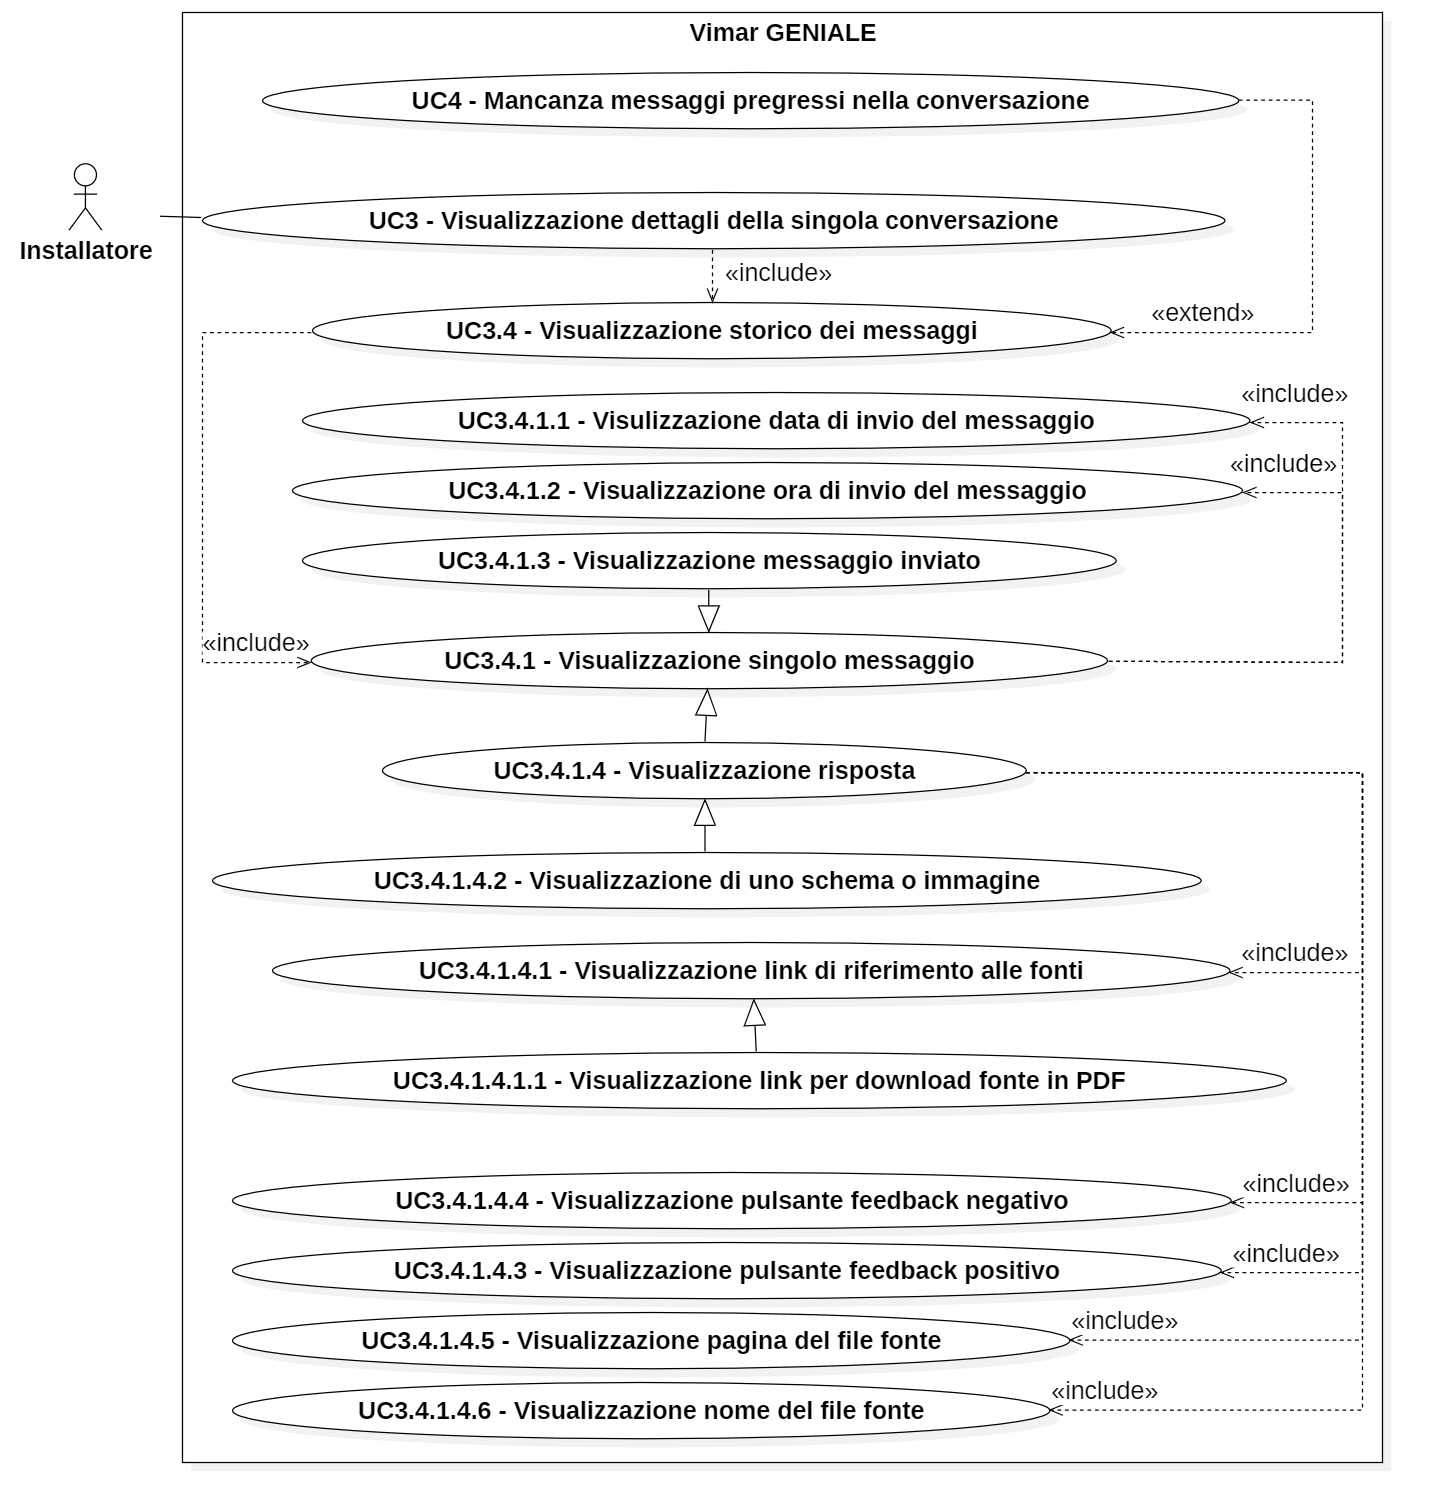
\includegraphics[width=1\textwidth]{contents/casi_duso/png/UC3.4.png}
\caption{UC3.4 - Visualizzazione storico dei messaggi}
% \label{fig:UC1a}
\end{figure}

\subsubuc{Visualizzazione singolo messaggio}{visual_msg}
\begin{itemize}
    \item \textbf{Attori coinvolti}: Installatore;
    \item \textbf{Descrizione}: L'installatore vuole visualizzare un singolo messaggio della conversazione selezionata;
    \item \textbf{Precondizioni}: 
    \begin{itemize}
        \item L’installatore ha accesso all’\textit{interfaccia web}\textsubscript{G} del \textit{sistema}\textsubscript{G};
        \item L’installatore ha accesso ad una conversazione memorizzabile nel \textit{sistema}\textsubscript{G};
        \item L'installatore ha posto una domanda al \textit{sistema}\textsubscript{G}.
    \end{itemize}
    \item \textbf{Postcondizioni}: L'installatore visualizza un singolo messaggio della conversazione da lui selezionata;
    \item \textbf{Scenario principale}:
    \begin{enumerate}
        \item L’installatore ha accesso all’\textit{interfaccia web}\textsubscript{G} del \textit{sistema}\textsubscript{G};
        \item L’installatore ha accesso ad una conversazione memorizzabile (o memorizzata) nel \textit{sistema}\textsubscript{G};
        \item L'installatore visualizza la conversazione selezionata;
        \item L'installatore visualizza un singolo messaggio della conversazione selezionata.
    \end{enumerate}
    \item \textbf{Inclusioni}: 
    \begin{itemize}
        \item UC3.4.1.1 - Visulizzazione data di invio del messaggio;
        \item UC3.4.1.2 - Visualizzazione ora di invio del messaggio.
    \end{itemize}
\end{itemize}

\subsubsubuc{Visualizzazione data di invio del messaggio}{visual_data}
\begin{itemize}
    \item \textbf{Attori coinvolti}: Installatore;
    \item \textbf{Descrizione}: L'installatore vuole visualizzare la data di invio di un determinato messaggio della conversazione;
    \item \textbf{Precondizioni}:  
    \begin{itemize}
        \item L’installatore ha accesso all’\textit{interfaccia web}\textsubscript{G} del \textit{sistema}\textsubscript{G};
        \item L’installatore ha accesso ad una conversazione memorizzabile nel \textit{sistema}\textsubscript{G};
        \item L'installatore ha posto una domanda al \textit{sistema}\textsubscript{G}.
    \end{itemize}
    \item \textbf{Postcondizioni}: L'installatore visualizza la data di invio del messaggio;
    \item \textbf{Scenario principale}:
    \begin{enumerate}
        \item L’installatore ha accesso all’\textit{interfaccia web}\textsubscript{G} del \textit{sistema}\textsubscript{G};
        \item L’installatore ha accesso ad una conversazione memorizzabile (o memorizzata) nel \textit{sistema}\textsubscript{G};
        \item L'installatore visualizza la data di invio del messaggio.
    \end{enumerate}
\end{itemize}

\subsubsubuc{Visualizzazione ora di invio del messaggio}{visual_ora}
\begin{itemize}
    \item \textbf{Attori coinvolti}: Installatore;
    \item \textbf{Descrizione}: L'installatore vuole visualizzare l'ora di invio di un determinato messaggio della conversazione;
    \item \textbf{Precondizioni}:  
    \begin{itemize}
        \item L’installatore ha accesso all’\textit{interfaccia web}\textsubscript{G} del \textit{sistema}\textsubscript{G};
        \item L’installatore ha accesso ad una conversazione memorizzabile nel \textit{sistema}\textsubscript{G};
        \item L'installatore ha posto una domanda al \textit{sistema}\textsubscript{G}.
    \end{itemize}
    \item \textbf{Postcondizioni}: L'installatore visualizza l'ora di invio del messaggio;
    \item \textbf{Scenario principale}:
    \begin{enumerate}
        \item L’installatore ha accesso all’\textit{interfaccia web}\textsubscript{G} del \textit{sistema}\textsubscript{G};
        \item L’installatore ha accesso ad una conversazione memorizzabile (o memorizzata) nel \textit{sistema}\textsubscript{G};
        \item L'installatore visualizza l'ora di invio del messaggio.
    \end{enumerate}
\end{itemize}

\subsubsubuc{Visualizzazione messaggio inviato}{visual_domanda}
\begin{itemize}
    \item \textbf{Attori coinvolti}: Installatore;
    \item \textbf{Descrizione}: L'installatore vuole visualizzare un singolo messaggio da lui inviato nella conversazione selezionata;
    \item \textbf{Precondizioni}: 
    \begin{itemize}
        \item L’installatore ha accesso all’\textit{interfaccia web}\textsubscript{G} del \textit{sistema}\textsubscript{G};
        \item L’installatore ha accesso ad una conversazione memorizzabile nel \textit{sistema}\textsubscript{G};
        \item L'installatore ha posto una domanda al \textit{sistema}\textsubscript{G}.
    \end{itemize}
    \item \textbf{Postcondizioni}: L'installatore visualizza un singolo messaggio che ha inviato nella conversazione da lui selezionata;
    \item \textbf{Scenario principale}:
    \begin{enumerate}
        \item L’installatore ha accesso all’\textit{interfaccia web}\textsubscript{G} del \textit{sistema}\textsubscript{G};
        \item L’installatore ha accesso ad una conversazione memorizzabile (o memorizzata) nel \textit{sistema}\textsubscript{G};
        \item L'installatore visualizza la conversazione selezionata;
        \item L'installatore visualizza un singolo messaggio da lui inviato nella conversazione selezionata.
    \end{enumerate}
    \item \textbf{Generalizzazioni}: UC3.4.1 - Visualizzazione singolo messaggio.
\end{itemize}

\subsubsubuc{Visualizzazione risposta}{visual_risposta}
\begin{itemize}
    \item \textbf{Attori coinvolti}: Installatore;
    \item \textbf{Descrizione}: L'installatore vuole visualizzare una singola risposta da lui ricevuta nella conversazione selezionata;
    \item \textbf{Precondizioni}: 
    \begin{itemize}
        \item L’installatore ha accesso all’\textit{interfaccia web}\textsubscript{G} del \textit{sistema}\textsubscript{G};
        \item L’installatore ha accesso ad una conversazione memorizzabile nel \textit{sistema}\textsubscript{G};
        \item L'installatore ha posto una domanda al \textit{sistema}\textsubscript{G};
        \item Il \textit{sistema}\textsubscript{G} ha fornito una risposta ad un’interrogazione da parte dell’installatore.
    \end{itemize}
    \item \textbf{Postcondizioni}: L'installatore visualizza una singola risposta che ha ricevuto nella conversazione da lui selezionata;
    \item \textbf{Scenario principale}:
    \begin{enumerate}
        \item L’installatore ha accesso all’\textit{interfaccia web}\textsubscript{G} del \textit{sistema}\textsubscript{G};
        \item L’installatore ha accesso ad una conversazione memorizzabile (o memorizzata) nel \textit{sistema}\textsubscript{G};
        \item L'installatore visualizza la conversazione selezionata;
        \item L'installatore visualizza una singola risposta da lui ricevuta nella conversazione selezionata.
    \end{enumerate}
    \item \textbf{Generalizzazioni}: UC3.4.1 - Visualizzazione singolo messaggio;
    \item \textbf{Inclusioni}: 
    \begin{itemize}
        \item UC3.4.1.4.1 - Visualizzazione link di riferimento alle fonti;
        \item UC3.4.1.4.3 - Visualizzazione pulsante feedback positivo;
        \item UC3.4.1.4.4 - Visualizzazione pulsante feedback negativo;
        \item UC3.4.1.4.5 - Visualizzazione pagina del file fonte;
        \item UC3.4.1.4.6 - Visualizzazione nome del file fonte.
    \end{itemize}
\end{itemize}

\subsubsubsubuc{Visualizzazione link di riferimento alle fonti}{visual_rif}
\begin{itemize}
    \item \textbf{Attori coinvolti}: Installatore;
    \item \textbf{Descrizione}: L'installatore vuole visualizzare un link che permetta di esaminare le fonti che sono state utilizzate per formulare la risposta fornita dal \textit{sistema}\textsubscript{G};
    \item \textbf{Precondizioni}: 
    \begin{itemize}
        \item L’installatore ha accesso all’\textit{interfaccia web}\textsubscript{G} del \textit{sistema}\textsubscript{G};
        \item L’installatore ha accesso ad una conversazione memorizzabile nel \textit{sistema}\textsubscript{G};
        \item L'installatore ha posto una domanda al \textit{sistema}\textsubscript{G};
        \item Il \textit{sistema}\textsubscript{G} ha fornito una risposta ad un’interrogazione da parte dell’installatore.
    \end{itemize}
    \item \textbf{Postcondizioni}: L'installatore visualizza un link che permette di esaminare le fonti che sono state utilizzate per formulare la risposta ricevuta;
    \item \textbf{Scenario principale}:
    \begin{enumerate}
        \item L’installatore ha accesso all’\textit{interfaccia web}\textsubscript{G} del \textit{sistema}\textsubscript{G};
        \item L’installatore ha accesso ad una conversazione memorizzabile (o memorizzata) nel \textit{sistema}\textsubscript{G};
        \item L'installatore visualizza la conversazione selezionata;
        \item L'installatore visualizza una singola risposta da lui ricevuta nella conversazione selezionata;
        \item L'installatore visualizza il link di riferimento alle fonti a partire dalle quali è stata formulata la risposta.
    \end{enumerate}
\end{itemize}

\subsubsubsubsubuc{Visualizzazione link per download fonte in PDF}{visual_rif_down}
\begin{itemize}
    \item \textbf{Attori coinvolti}: Installatore;
    \item \textbf{Descrizione}: L'installatore vuole visualizzare un link che permetta di scaricare il documento che è stato utilizzato per formulare la risposta fornita dal \textit{sistema}\textsubscript{G};
    \item \textbf{Precondizioni}: 
    \begin{itemize}
        \item L’installatore ha accesso all’\textit{interfaccia web}\textsubscript{G} del \textit{sistema}\textsubscript{G};
        \item L’installatore ha accesso ad una conversazione memorizzabile nel \textit{sistema}\textsubscript{G};
        \item L'installatore ha posto una domanda al \textit{sistema}\textsubscript{G};
        \item Il \textit{sistema}\textsubscript{G} ha fornito una risposta ad un’interrogazione da parte dell’installatore, utilizzando un documento come fonte.
    \end{itemize}
    \item \textbf{Postcondizioni}: L'installatore visualizza un link che permette di scaricare il documento che è stato utilizzato per formulare la risposta ricevuta;
    \item \textbf{Scenario principale}:
    \begin{enumerate}
        \item L’installatore ha accesso all’\textit{interfaccia web}\textsubscript{G} del \textit{sistema}\textsubscript{G};
        \item L’installatore ha accesso ad una conversazione memorizzabile (o memorizzata) nel \textit{sistema}\textsubscript{G};
        \item L'installatore visualizza la conversazione selezionata;
        \item L'installatore visualizza una singola risposta da lui ricevuta nella conversazione selezionata;
        \item L'installatore visualizza il link che permette di scaricare il documento a partire dal quale è stata formulata la risposta.
    \end{enumerate}
    \item \textbf{Generalizzazioni}: UC3.4.1.4.1 - Visualizzazione link di riferimento alle fonti
\end{itemize}

\subsubsubsubuc{Visualizzazione di uno schema o immagine}{visual_img}
\begin{itemize}
    \item \textbf{Attori coinvolti}: Installatore;
    \item \textbf{Descrizione}: L'installatore vuole visualizzare una  risposta da lui ricevuta nella conversazione selezionata che contenga anche uno schema o un immagine;
    \item \textbf{Precondizioni}: 
    \begin{itemize}
        \item L’installatore ha accesso all’\textit{interfaccia web}\textsubscript{G} del \textit{sistema}\textsubscript{G};
        \item L’installatore ha accesso ad una conversazione memorizzabile nel \textit{sistema}\textsubscript{G};
        \item L'installatore ha posto una domanda al \textit{sistema}\textsubscript{G}, richiedendo anche degli schemi o immagini specifici;
        \item Il \textit{sistema}\textsubscript{G} ha fornito una risposta all’interrogazione da parte dell’installatore.
    \end{itemize}
    \item \textbf{Postcondizioni}: L'installatore visualizza una risposta ricevuta nella conversazione da lui selezionata che contenga anche uno schema o un immagine;
    \item \textbf{Scenario principale}:
    \begin{enumerate}
        \item L’installatore ha accesso all’\textit{interfaccia web}\textsubscript{G} del \textit{sistema}\textsubscript{G};
        \item L’installatore ha accesso ad una conversazione memorizzabile (o memorizzata) nel \textit{sistema}\textsubscript{G};
        \item L'installatore visualizza la conversazione selezionata;
        \item L'installatore visualizza la risposta da lui ricevuta nella conversazione selezionata;
        \item L'installatore visualizza lo schema o l'immagine restituiti dal \textit{sistema}\textsubscript{G} con la risposta.
    \end{enumerate}
    \item \textbf{Generalizzazioni}: UC3.4.1.4 - Visualizzazione risposta.
\end{itemize}

\subsubsubsubuc{Visualizzazione pulsante feedback positivo}{visual_feedback_pos}
\begin{itemize}
    \item \textbf{Attori coinvolti}: Installatore;
    \item \textbf{Descrizione}: L'installatore vuole visualizzare un pulsante che permetta di fornire un feedback positivo per la risposta restituita dal \textit{sistema}\textsubscript{G};
    \item \textbf{Precondizioni}: 
    \begin{itemize}
        \item L’installatore ha accesso all’\textit{interfaccia web}\textsubscript{G} del \textit{sistema}\textsubscript{G};
        \item L’installatore ha accesso ad una conversazione memorizzabile nel \textit{sistema}\textsubscript{G};
        \item L'installatore ha posto una domanda al \textit{sistema}\textsubscript{G};
        \item Il \textit{sistema}\textsubscript{G} ha fornito una risposta ad un’interrogazione da parte dell’installatore.
    \end{itemize}
    \item \textbf{Postcondizioni}: L'installatore visualizza un pulsante che permetta di fornire un feedback positivo per la risposta ricevuta;
    \item \textbf{Scenario principale}:
    \begin{enumerate}
        \item L’installatore ha accesso all’\textit{interfaccia web}\textsubscript{G} del \textit{sistema}\textsubscript{G};
        \item L’installatore ha accesso ad una conversazione memorizzabile (o memorizzata) nel \textit{sistema}\textsubscript{G};
        \item L'installatore visualizza la conversazione selezionata;
        \item L'installatore visualizza una singola risposta da lui ricevuta nella conversazione selezionata;
        \item L'installatore visualizza il pulsante che permette di fornire un feedback positivo per la risposta.
    \end{enumerate}
\end{itemize}

\subsubsubsubuc{Visualizzazione pulsante feedback negativo}{visual_feedback_pos}
\begin{itemize}
    \item \textbf{Attori coinvolti}: Installatore;
    \item \textbf{Descrizione}: L'installatore vuole visualizzare un pulsante che permetta di fornire un feedback negativo per la risposta restituita dal \textit{sistema}\textsubscript{G};
    \item \textbf{Precondizioni}: 
    \begin{itemize}
        \item L’installatore ha accesso all’\textit{interfaccia web}\textsubscript{G} del \textit{sistema}\textsubscript{G};
        \item L’installatore ha accesso ad una conversazione memorizzabile nel \textit{sistema}\textsubscript{G};
        \item L'installatore ha posto una domanda al \textit{sistema}\textsubscript{G};
        \item Il \textit{sistema}\textsubscript{G} ha fornito una risposta ad un’interrogazione da parte dell’installatore.
    \end{itemize}
    \item \textbf{Postcondizioni}: L'installatore visualizza un pulsante che permetta di fornire un feedback negativo per la risposta ricevuta;
    \item \textbf{Scenario principale}:
    \begin{enumerate}
        \item L’installatore ha accesso all’\textit{interfaccia web}\textsubscript{G} del \textit{sistema}\textsubscript{G};
        \item L’installatore ha accesso ad una conversazione memorizzabile (o memorizzata) nel \textit{sistema}\textsubscript{G};
        \item L'installatore visualizza la conversazione selezionata;
        \item L'installatore visualizza una singola risposta da lui ricevuta nella conversazione selezionata;
        \item L'installatore visualizza il pulsante che permette di fornire un feedback negativo per la risposta.
    \end{enumerate}
\end{itemize}

\subsubsubsubuc{Visualizzazione pagina del file fonte}{visual_pag_rif}
\begin{itemize}
    \item \textbf{Attori coinvolti}: Installatore;
    \item \textbf{Descrizione}: L'installatore vuole visualizzare il numero della pagina del documento che è stata utilizzata per formulare la risposta fornita dal \textit{sistema}\textsubscript{G};
    \item \textbf{Precondizioni}: 
    \begin{itemize}
        \item L’installatore ha accesso all’\textit{interfaccia web}\textsubscript{G} del \textit{sistema}\textsubscript{G};
        \item L’installatore ha accesso ad una conversazione memorizzabile nel \textit{sistema}\textsubscript{G};
        \item L'installatore ha posto una domanda al \textit{sistema}\textsubscript{G};
        \item Il \textit{sistema}\textsubscript{G} ha fornito una risposta ad un’interrogazione da parte dell’installatore.
    \end{itemize}
    \item \textbf{Postcondizioni}: L'installatore visualizza il numero dalla pagina del documento che è stata utilizzata per formulare la risposta ricevuta;
    \item \textbf{Scenario principale}:
    \begin{enumerate}
        \item L’installatore ha accesso all’\textit{interfaccia web}\textsubscript{G} del \textit{sistema}\textsubscript{G};
        \item L’installatore ha accesso ad una conversazione memorizzabile (o memorizzata) nel \textit{sistema}\textsubscript{G};
        \item L'installatore visualizza la conversazione selezionata;
        \item L'installatore visualizza una singola risposta da lui ricevuta nella conversazione selezionata;
        \item L'installatore visualizza il numero della pagina del documento a partire dalla quale è stata formulata la risposta.
    \end{enumerate}
\end{itemize}

\subsubsubsubuc{Visualizzazione nome del file fonte}{visual_nome_rif}
\begin{itemize}
    \item \textbf{Attori coinvolti}: Installatore;
    \item \textbf{Descrizione}: L'installatore vuole visualizzare il nome del documento che è stato utilizzato per formulare la risposta fornita dal \textit{sistema}\textsubscript{G};
    \item \textbf{Precondizioni}: 
    \begin{itemize}
        \item L’installatore ha accesso all’\textit{interfaccia web}\textsubscript{G} del \textit{sistema}\textsubscript{G};
        \item L’installatore ha accesso ad una conversazione memorizzabile nel \textit{sistema}\textsubscript{G};
        \item L'installatore ha posto una domanda al \textit{sistema}\textsubscript{G};
        \item Il \textit{sistema}\textsubscript{G} ha fornito una risposta ad un’interrogazione da parte dell’installatore.
    \end{itemize}
    \item \textbf{Postcondizioni}: L'installatore visualizza il nome del documento che è stato utilizzato per formulare la risposta ricevuta;
    \item \textbf{Scenario principale}:
    \begin{enumerate}
        \item L’installatore ha accesso all’\textit{interfaccia web}\textsubscript{G} del \textit{sistema}\textsubscript{G};
        \item L’installatore ha accesso ad una conversazione memorizzabile (o memorizzata) nel \textit{sistema}\textsubscript{G};
        \item L'installatore visualizza la conversazione selezionata;
        \item L'installatore visualizza una singola risposta da lui ricevuta nella conversazione selezionata;
        \item L'installatore visualizza il nome del documento a partire dal quale è stata formulata la risposta.
    \end{enumerate}
\end{itemize}

\uc{Mancanza messaggi pregressi nella conversazione}{mancanza_messaggi_pregressi}
\begin{itemize}
    \item \textbf{Attori coinvolti}: Installatore;
    \item \textbf{Descrizione}: L’installatore vuole visualizzare lo storico dei messaggi di una conversazione o il suggerimento per la prossima domanda da porre al sistema, ma non ci sono messaggi pregressi nella conversazione attuale;
    \item \textbf{Precondizioni}: 
    \begin{itemize}
        \item L’installatore ha accesso all’\textit{interfaccia web}\textsubscript{G} del \textit{sistema}\textsubscript{G};
        \item L’installatore ha accesso ad una conversazione memorizzabile nel \textit{sistema}\textsubscript{G};
        \item La conversazione attuale non contiene messaggi scambiati in precedenza.
    \end{itemize}
    \item \textbf{Postcondizioni}: Il \textit{sistema}\textsubscript{G} restituisce una risposta che indica l’assenza di messaggi pregressi nella conversazione attuale;
    \item \textbf{Scenario principale}:
    \begin{enumerate}
        \item L’installatore accede all’\textit{interfaccia web}\textsubscript{G} di Vimar GENIALE;
        \item Accede ad una conversazione presente nel \textit{sistema}\textsubscript{G} e richiede di visualizzarne uno storico dei messaggi o di visualizzare il suggerimento per la prossima domanda da porre al sistema;
        \item Il \textit{sistema}\textsubscript{G} elabora la richiesta e fornisce una risposta che indica l’assenza di messaggi pregressi nella conversazione attuale;
        \item L’installatore visualizza il messaggio che indica l’assenza di messaggi pregressi.
    \end{enumerate}
\end{itemize}



\uc{Ricerca informazioni sui prodotti}{ricerca_info_prodotti}
\begin{itemize}
    \item \textbf{Attori coinvolti}: Installatore;
    \item \textbf{Descrizione}: L’installatore interroga il \textit{sistema}\textsubscript{G} per ottenere informazioni dettagliate su un prodotto specifico, come schemi elettrici, dati tecnici e manuali;
    \item \textbf{Precondizioni}: 
    \begin{itemize}
        \item L’installatore ha accesso all’\textit{interfaccia web}\textsubscript{G} del \textit{sistema}\textsubscript{G};
        \item L’installatore ha accesso ad una conversazione memorizzabile nel \textit{sistema}\textsubscript{G};
        \item Il prodotto richiesto è registrato nel \textit{sistema}\textsubscript{G} e le informazioni sono correttamente indicizzate.
    \end{itemize}
    \item \textbf{Postcondizioni}: Il \textit{sistema}\textsubscript{G} restituisce le informazioni richieste, incluse le descrizioni del prodotto, schemi elettrici e manuali di configurazione;
    \item \textbf{Scenario principale}:
    \begin{enumerate}
        \item L’installatore accede all’\textit{interfaccia web}\textsubscript{G} di Vimar GENIALE;
        \item Inserisce una domanda o una parola chiave relativa ad un prodotto specifico;
        \item Il \textit{sistema}\textsubscript{G} esegue la ricerca nel \textit{database}\textsubscript{G} le informazioni necessarie a fornire sufficiente contesto al \textit{LLM}\textsubscript{G}.
    \end{enumerate}
    \item \textbf{Inclusioni}: UC5.1 - Domanda al sistema;
    \item \textbf{Estensioni}: 
    \begin{itemize}
        \item UC6 - Richiesta di argomento proibito;
        \item UC7 - Assenza di informazioni sul prodotto ricercato.
    \end{itemize}
\end{itemize}
\begin{figure}[H]
\centering
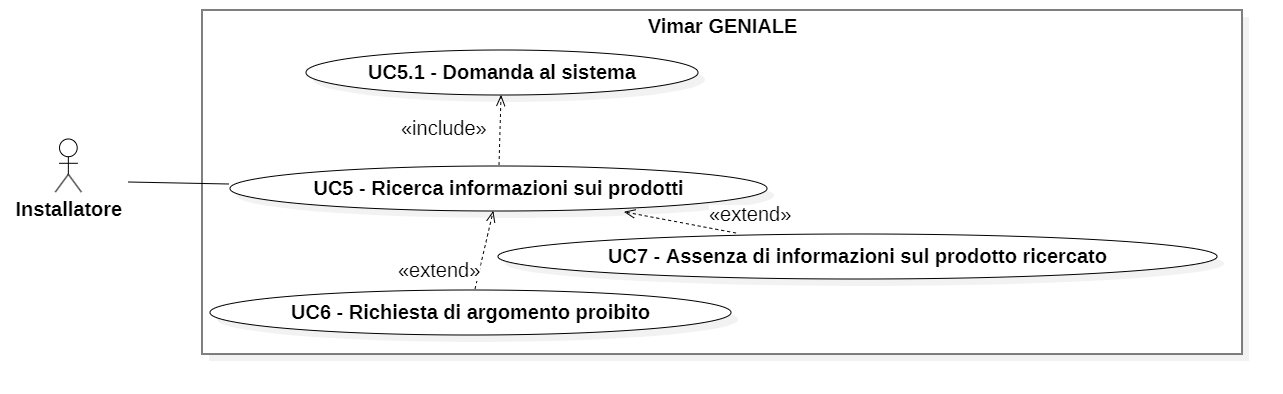
\includegraphics[width=1\textwidth]{contents/casi_duso/png/UC5.png}
\caption{UC5 - Ricerca informazioni sui prodotti}
% \label{fig:UC1a}
\end{figure}

\subuc{Domanda al sistema\textsubscript{G}}{domanda}
\begin{itemize}
    \item \textbf{Attori coinvolti}: Installatore;
    \item \textbf{Descrizione}: L’installatore inserisce una domanda che verrà elaborata dal \textit{sistema}\textsubscript{G};
    \item \textbf{Precondizioni}: 
    \begin{itemize}
        \item L’installatore ha accesso all’\textit{interfaccia web}\textsubscript{G} del \textit{sistema}\textsubscript{G};
        \item L’installatore ha accesso ad una conversazione memorizzabile nel \textit{sistema}\textsubscript{G};
        \item L'installatore ha inviato una domanda al \textit{sistema}\textsubscript{G};
        \item La domanda posta non riguarda argomenti proibiti.
    \end{itemize}
    \item \textbf{Postcondizioni}: Il \textit{sistema}\textsubscript{G} restituisce una risposta;
    \item \textbf{Scenario principale}:
    \begin{enumerate}
        \item L’installatore accede all’\textit{interfaccia web}\textsubscript{G} di Vimar GENIALE;
        \item Inserisce una domanda che ha a che vedere con prodotti \textit{VIMAR}\textsubscript{G} e non con argomenti proibiti o sconosciuti;
        \item Il \textit{sistema}\textsubscript{G} elabora la richiesta e fornisce una risposta;
        \item L’installatore visualizza le informazioni restituite.
    \end{enumerate}
\end{itemize}
\begin{figure}[H]
\centering
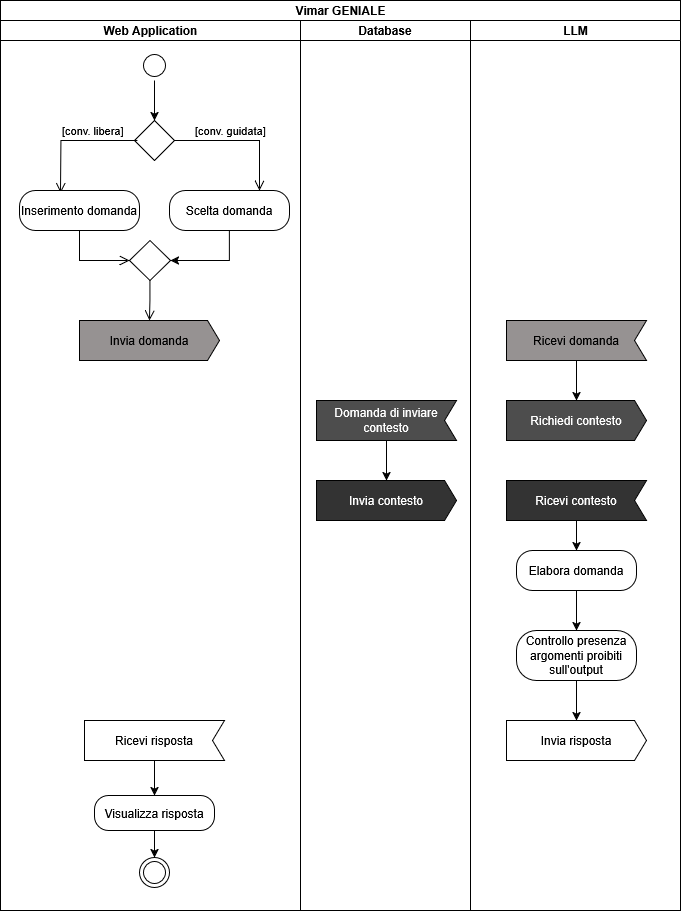
\includegraphics[width=0.8\textwidth]{contents/casi_duso/png/UC5.1_activity.png}
\caption{UC5.1 - Domanda al \textit{sistema}\textsubscript{G}}
% \label{fig:UC1a}
\end{figure}

\uc{Richiesta di argomento proibito}{argomento_proibito}
\begin{itemize}
    \item \textbf{Attori coinvolti}: Installatore;
    \item \textbf{Descrizione}: L’installatore richiede argomenti proibiti al \textit{sistema}\textsubscript{G} (e.g. politica, finanza, pornografia, ...);
    \item \textbf{Precondizioni}: 
    \begin{itemize}
        \item L’installatore ha accesso all’\textit{interfaccia web}\textsubscript{G} del \textit{sistema}\textsubscript{G};
        \item L’installatore ha accesso ad una conversazione memorizzabile nel \textit{sistema}\textsubscript{G};
        \item La domanda posta riguarda argomenti proibiti.
    \end{itemize}
    \item \textbf{Postcondizioni}: Il \textit{sistema}\textsubscript{G} restituisce una risposta che indica il motivo per cui si è verificato l’errore;
    \item \textbf{Scenario principale}:
    \begin{enumerate}
        \item L’installatore accede all’\textit{interfaccia web}\textsubscript{G} di Vimar GENIALE;
        \item Inserisce una domanda inconsistente, che non ha a che vedere con prodotti \textit{VIMAR}\textsubscript{G};
        \item Il \textit{sistema}\textsubscript{G} elabora la richiesta e fornisce una risposta che spiega la causa dell'errore riscontrato;
        \item L’installatore visualizza le informazioni sull’errore che si è verificato.
    \end{enumerate}
\end{itemize}

\uc{Assenza di informazioni sul prodotto ricercato}{assenza_info_prodotto}
\begin{itemize}
    \item \textbf{Attori coinvolti}: Installatore;
    \item \textbf{Descrizione}: L’installatore interroga il \textit{sistema}\textsubscript{G} per ottenere informazioni dettagliate su un prodotto specifico, ma il \textit{sistema}\textsubscript{G} non è in grado di trovare nessuna informazione relativa ad esso;
    \item \textbf{Precondizioni}: 
    \begin{itemize}
        \item L’installatore ha accesso all’\textit{interfaccia web}\textsubscript{G} del \textit{sistema}\textsubscript{G};
        \item L’installatore ha accesso ad una conversazione memorizzabile nel \textit{sistema}\textsubscript{G};
        \item L’installatore pone una domanda al \textit{sistema}\textsubscript{G};
        \item Il \textit{sistema}\textsubscript{G} non è in possesso di alcuna informazione relativa al prodotto ricercato.
    \end{itemize}
    \item \textbf{Postcondizioni}: Il \textit{sistema}\textsubscript{G} restituisce una risposta che indica il motivo per cui si è verificato l’errore;
    \item \textbf{Scenario principale}:
    \begin{enumerate}
        \item L’installatore accede all’\textit{interfaccia web}\textsubscript{G} di Vimar GENIALE;
        \item Inserisce una domanda o una parola chiave relativa ad un prodotto specifico;
        \item Il \textit{sistema}\textsubscript{G} elabora la richiesta e fornisce una risposta che spiega la causa dell'errore riscontrato;
        \item L’installatore visualizza le informazioni sull’errore che si è verificato.
    \end{enumerate}
\end{itemize}



\uc{Digitazione della domanda}{digita_domanda}
\begin{itemize}
    \item \textbf{Attori coinvolti}: Installatore;
    \item \textbf{Descrizione}: L’installatore inserisce una domanda;
    \item \textbf{Precondizioni}: 
    \begin{itemize}
        \item L’installatore ha accesso all’\textit{interfaccia web}\textsubscript{G} del \textit{sistema}\textsubscript{G};
        \item L’installatore ha accesso ad una conversazione memorizzabile nel \textit{sistema}\textsubscript{G}.
    \end{itemize}
    \item \textbf{Postcondizioni}: L'installatore invia la domanda al \textit{sistema}\textsubscript{G};
    \item \textbf{Scenario principale}:
    \begin{enumerate}
        \item L’installatore accede all’\textit{interfaccia web}\textsubscript{G} di Vimar GENIALE;
        \item Inserisce una domanda;
        \item Il \textit{sistema}\textsubscript{G} riceve la domanda ed inizia ad elaborarla.
    \end{enumerate}
    \item \textbf{Estensioni}: UC9 - Superamento limite di caratteri del messaggio.
\end{itemize}
\begin{figure}[H]
\centering
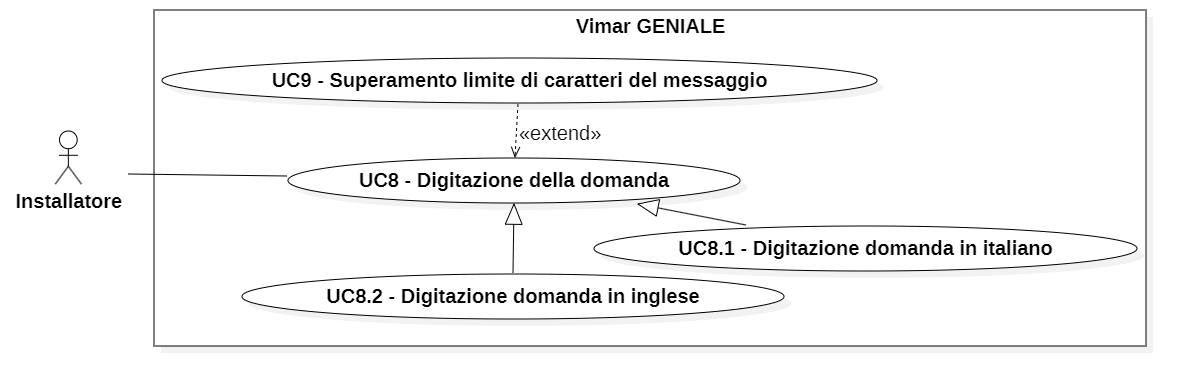
\includegraphics[width=1\textwidth]{contents/casi_duso/png/UC8.png}
\caption{UC8 - Digitazione della domanda}
% \label{fig:UC1a}
\end{figure}

\subuc{Digitazione domanda in italiano}{digita_domanda_ita}
\begin{itemize}
    \item \textbf{Attori coinvolti}: Installatore;
    \item \textbf{Descrizione}: L’installatore inserisce una domanda in lingua italiana;
    \item \textbf{Precondizioni}: 
    \begin{itemize}
        \item L’installatore ha accesso all’\textit{interfaccia web}\textsubscript{G} del \textit{sistema}\textsubscript{G};
        \item L’installatore ha accesso ad una conversazione memorizzabile nel \textit{sistema}\textsubscript{G}.
    \end{itemize}
    \item \textbf{Postcondizioni}: L'installatore invia la domanda al \textit{sistema}\textsubscript{G};
    \item \textbf{Scenario principale}:
    \begin{enumerate}
        \item L’installatore accede all’\textit{interfaccia web}\textsubscript{G} di Vimar GENIALE;
        \item Inserisce una domanda in lingua italiana;
        \item Il \textit{sistema}\textsubscript{G} riceve la domanda ed inizia ad elaborarla.
    \end{enumerate}
\end{itemize}

\subuc{Digitazione domanda in inglese}{digita_domanda_eng}
\begin{itemize}
    \item \textbf{Attori coinvolti}: Installatore;
    \item \textbf{Descrizione}: L’installatore inserisce una domanda in lingua inglese;
    \item \textbf{Precondizioni}: 
    \begin{itemize}
        \item L’installatore ha accesso all’\textit{interfaccia web}\textsubscript{G} del \textit{sistema}\textsubscript{G};
        \item L’installatore ha accesso ad una conversazione memorizzabile nel \textit{sistema}\textsubscript{G}.
    \end{itemize}
    \item \textbf{Postcondizioni}: L'installatore invia la domanda al \textit{sistema}\textsubscript{G};
    \item \textbf{Scenario principale}:
    \begin{enumerate}
        \item L’installatore accede all’\textit{interfaccia web}\textsubscript{G} di Vimar GENIALE;
        \item Inserisce una domanda in lingua inglese;
        \item Il \textit{sistema}\textsubscript{G} riceve la domanda ed inizia ad elaborarla.
    \end{enumerate}
\end{itemize}

\uc{Superamento limite caratteri del messaggio}{superamento_limite_caratteri}
\begin{itemize}
    \item \textbf{Attori coinvolti}: Installatore;
    \item \textbf{Descrizione}: L’installatore, quando interroga il \textit{sistema}\textsubscript{G} per ottenere informazioni, supera il limite di caratteri che possono essere utilizzati per effettuare la richiesta;
    \item \textbf{Precondizioni}: 
    \begin{itemize}
        \item L’installatore ha accesso all’\textit{interfaccia web}\textsubscript{G} del \textit{sistema}\textsubscript{G};
        \item L’installatore ha accesso ad una conversazione memorizzabile nel \textit{sistema}\textsubscript{G};
        \item La domanda posta supera il limite massimo di caratteri consentiti.
    \end{itemize}
    \item \textbf{Postcondizioni}: Il \textit{sistema}\textsubscript{G} restituisce una risposta che indica il motivo per cui si è verificato l’errore;
    \item \textbf{Scenario principale}:
    \begin{enumerate}
        \item L’installatore accede all’\textit{interfaccia web}\textsubscript{G} di Vimar GENIALE;
        \item Inserisce una domanda o una parola chiave relativa ad un prodotto specifico, superando il limite massimo consentito di caratteri;
        \item Il \textit{sistema}\textsubscript{G} elabora la richiesta e fornisce una risposta che spiega la causa dell'errore riscontrato;
        \item L’installatore visualizza le informazioni sull’errore che si è verificato.
    \end{enumerate}
\end{itemize}



\uc{Fornitura di \textit{feedback}\textsubscript{G} sulla risposta del \textit{sistema}\textsubscript{G} ad interrogazione}{fornitura_feedback}
\begin{itemize}
    \item \textbf{Attori coinvolti}: Installatore;
    \item \textbf{Descrizione}: L’installatore, a seguito dell’interrogazione del \textit{sistema}\textsubscript{G} per ottenere informazioni, desidera fornire un \textit{feedback}\textsubscript{G} che indichi se la risposta ricevuta sia corretta o meno;
    \item \textbf{Precondizioni}: 
    \begin{itemize}
        \item L’installatore ha accesso all’\textit{interfaccia web}\textsubscript{G} del \textit{sistema}\textsubscript{G};
        \item L’installatore ha accesso ad una conversazione memorizzabile nel \textit{sistema}\textsubscript{G};
        \item Il \textit{sistema}\textsubscript{G} fornisce una risposta ad un’interrogazione da parte dell’installatore.
    \end{itemize}
    \item \textbf{Postcondizioni}: L’installatore, dopo aver esaminato la risposta ricevuta, fornisce un riscontro sulla correttezza di quest’ultima che verrà registrato dal \textit{sistema}\textsubscript{G};
    \item \textbf{Scenario principale}:
    \begin{enumerate}
        \item L’installatore accede all’\textit{interfaccia web}\textsubscript{G} di Vimar GENIALE;
        \item Inserisce una domanda o una parola chiave relativa ad un prodotto specifico;
        \item Il \textit{sistema}\textsubscript{G} esegue la ricerca nel \textit{database}\textsubscript{G} dei prodotti e restituisce una risposta che include informazioni dettagliate come schemi, descrizioni e manuali;
        \item L’installatore visualizza le informazioni fornite e, dopo aver verificato la correttezza delle informazioni ricevute, fornisce un \textit{feedback}\textsubscript{G} sulla risposta al \textit{sistema}\textsubscript{G};
        \item Il \textit{sistema}\textsubscript{G} registra il \textit{feedback}\textsubscript{G} ricevuto dall’installatore.
    \end{enumerate}
\end{itemize}
\begin{figure}[H]
\centering
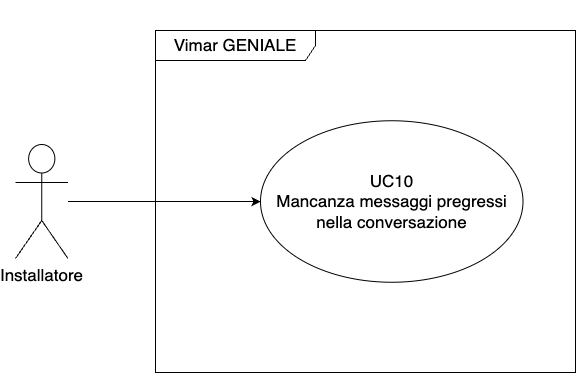
\includegraphics[width=1\textwidth]{contents/casi_duso/png/UC10.png}
\caption{UC10 - Fornitura di \textit{feedback}\textsubscript{G} sulla risposta del \textit{sistema}\textsubscript{G} ad interrogazione}
% \label{fig:UC1a}
\end{figure}

\subuc{Fornitura di \textit{feedback}\textsubscript{G} positivo sulla risposta del \textit{sistema}\textsubscript{G} ad interrogazione}{feedback_positivo}
\begin{itemize}
    \item \textbf{Attori coinvolti}: Installatore;
    \item \textbf{Descrizione}: L’installatore, a seguito dell’interrogazione del \textit{sistema}\textsubscript{G} per ottenere informazioni, desidera fornire un \textit{feedback}\textsubscript{G} che indichi che la risposta ricevuta è corretta;
    \item \textbf{Precondizioni}: 
    \begin{itemize}
        \item L’installatore ha accesso all’\textit{interfaccia web}\textsubscript{G} del \textit{sistema}\textsubscript{G};
        \item L’installatore ha accesso ad una conversazione memorizzabile nel \textit{sistema}\textsubscript{G};
        \item Il \textit{sistema}\textsubscript{G} fornisce una risposta corretta ad un’interrogazione da parte dell’installatore.
    \end{itemize}
    \item \textbf{Postcondizioni}: L’installatore, dopo aver esaminato la risposta ricevuta, fornisce un riscontro positivo sulla correttezza di quest’ultima che verrà registrato dal \textit{sistema}\textsubscript{G};
    \item \textbf{Scenario principale}:
    \begin{enumerate}
        \item L’installatore accede all’\textit{interfaccia web}\textsubscript{G} di Vimar GENIALE;
        \item Inserisce una domanda o una parola chiave relativa ad un prodotto specifico;
        \item Il \textit{sistema}\textsubscript{G} esegue la ricerca nel \textit{database}\textsubscript{G} dei prodotti e restituisce una risposta che include informazioni dettagliate come schemi, descrizioni e manuali;
        \item L’installatore visualizza le informazioni fornite e, dopo aver verificato la correttezza delle informazioni ricevute, fornisce un \textit{feedback}\textsubscript{G} positivo sulla risposta al \textit{sistema}\textsubscript{G};
        \item Il \textit{sistema}\textsubscript{G} registra il \textit{feedback}\textsubscript{G} ricevuto dall’installatore.
    \end{enumerate}
    \item \textbf{Generalizzazioni}: UC10 - Fornitura di \textit{feedback}\textsubscript{G} sulla risposta del sistema ad interrogazione.
\end{itemize}

\subuc{Fornitura di \textit{feedback}\textsubscript{G} negativo sulla risposta del \textit{sistema}\textsubscript{G} ad interrogazione}{feedback_negativo}
\begin{itemize}
    \item \textbf{Attori coinvolti}: Installatore;
    \item \textbf{Descrizione}: L’installatore, a seguito dell’interrogazione del \textit{sistema}\textsubscript{G} per ottenere informazioni, desidera fornire un \textit{feedback}\textsubscript{G} che indichi che la risposta ricevuta è errata;
    \item \textbf{Precondizioni}: 
    \begin{itemize}
        \item L’installatore ha accesso all’\textit{interfaccia web}\textsubscript{G} del \textit{sistema}\textsubscript{G};
        \item L’installatore ha accesso ad una conversazione memorizzata nel \textit{sistema}\textsubscript{G};
        \item Il \textit{sistema}\textsubscript{G} fornisce una risposta errata ad un’interrogazione da parte dell’installatore.
    \end{itemize}
    \item \textbf{Postcondizioni}: L’installatore, dopo aver esaminato la risposta ricevuta, fornisce un riscontro negativo sulla correttezza di quest’ultima che verrà registrato dal \textit{sistema}\textsubscript{G};
    \item \textbf{Scenario principale}:
    \begin{enumerate}
        \item L’installatore accede all’\textit{interfaccia web}\textsubscript{G} di Vimar GENIALE;
        \item Inserisce una domanda o una parola chiave relativa ad un prodotto specifico;
        \item Il \textit{sistema}\textsubscript{G} esegue la ricerca nel \textit{database}\textsubscript{G} dei prodotti e restituisce una risposta che include informazioni dettagliate come schemi, descrizioni e manuali;
        \item L’installatore visualizza le informazioni fornite e, dopo aver verificato la correttezza delle informazioni ricevute, fornisce un \textit{feedback}\textsubscript{G} negativo sulla risposta al \textit{sistema}\textsubscript{G};
        \item Il \textit{sistema}\textsubscript{G} registra il \textit{feedback}\textsubscript{G} ricevuto dall’installatore.
    \end{enumerate}
    \item \textbf{Generalizzazioni}: UC10 - Fornitura di \textit{feedback}\textsubscript{G} sulla risposta del sistema ad interrogazione.
\end{itemize}



\uc{Cancellazione conversazione}{cancellazione_conv}
\begin{itemize}
    \item \textbf{Attori coinvolti}: Installatore;
    \item \textbf{Descrizione}: L’installatore desidera eliminare una conversazione esistente, in quanto non è ritenuta più necessaria al suo scopo;
    \item \textbf{Precondizioni}: 
    \begin{itemize}
        \item L’installatore ha accesso all’\textit{interfaccia web}\textsubscript{G} del \textit{sistema}\textsubscript{G};
        \item L’installatore ha accesso ad una conversazione memorizzata nel \textit{sistema}\textsubscript{G}.
    \end{itemize}
    \item \textbf{Postcondizioni}: Il \textit{sistema}\textsubscript{G} elimina la conversazione non ritenuta più necessaria dall’installatore;
    \item \textbf{Scenario principale}:
    \begin{enumerate}
        \item L’installatore accede all’\textit{interfaccia web}\textsubscript{G} di Vimar GENIALE;
        \item Richiede l’eliminazione di una conversazione, in quanto ha raggiunto il suo scopo e non è più utile;
        \item Il \textit{sistema}\textsubscript{G} effettua l’eliminazione e fornisce una risposta che conferma il completamento dell’operazione;
        \item L’installatore visualizza il messaggio di conferma dell’avvenuta cancellazione.
    \end{enumerate}
\end{itemize}
\begin{figure}[H]
\centering
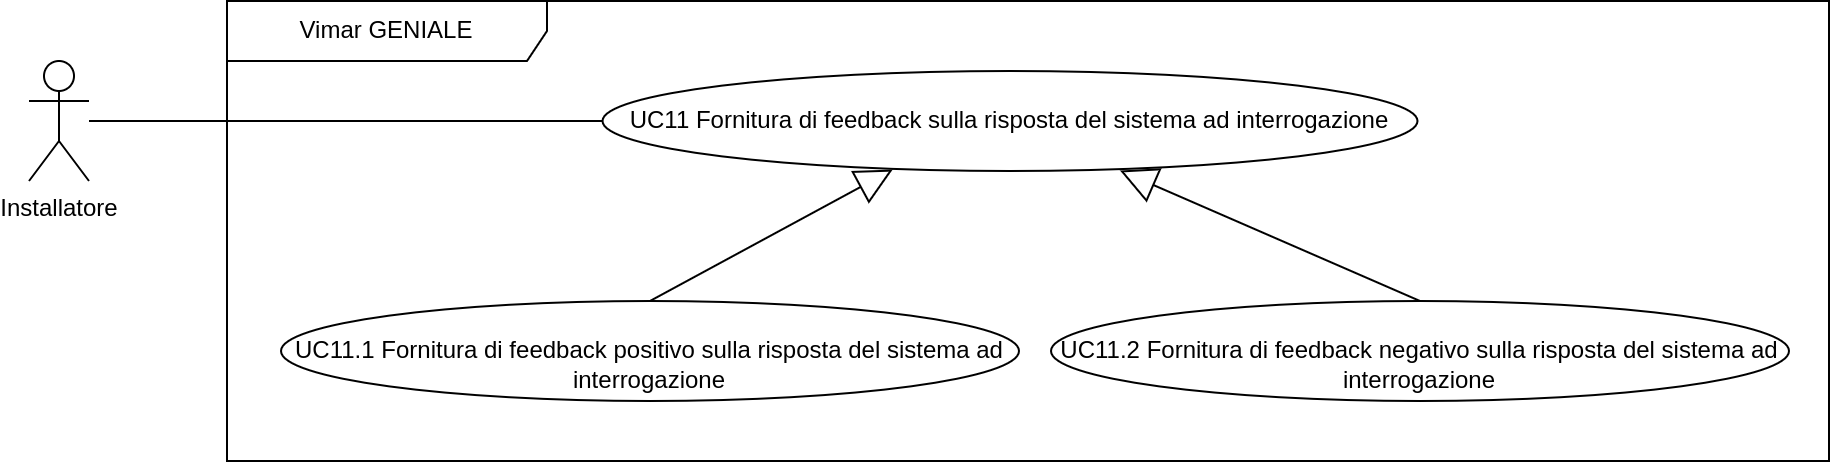
\includegraphics[width=1\textwidth]{contents/casi_duso/png/UC11.png}
\caption{UC11 - Cancellazione conversazione}
% \label{fig:UC1a}
\end{figure}



\uc{Salvataggio conversazione}{salvataggio_conv}
\begin{itemize}
    \item \textbf{Attori coinvolti}: Installatore;
    \item \textbf{Descrizione}: L’installatore, prima di chiudere l’applicativo, desidera salvare una conversazione memorizzata attualmente all’interno del \textit{sistema}\textsubscript{G}, per poterla consultare dopo aver chiuso l'applicativo;
    \item \textbf{Precondizioni}: 
    \begin{itemize}
        \item L’installatore ha accesso all’\textit{interfaccia web}\textsubscript{G} del \textit{sistema}\textsubscript{G};
        \item L’installatore ha accesso ad una conversazione memorizzabile nel \textit{sistema}\textsubscript{G}.
    \end{itemize}
    \item \textbf{Postcondizioni}: Il \textit{sistema}\textsubscript{G} salva la conversazione selezionata e memorizzata attualmente all’interno del \textit{sistema}\textsubscript{G};
    \item \textbf{Scenario principale}:
    \begin{enumerate}
        \item L’installatore accede all’\textit{interfaccia web}\textsubscript{G} di Vimar GENIALE;
        \item Richiede il salvataggio di una conversazione memorizzata attualmente all'interno del sistema;
        \item Il \textit{sistema}\textsubscript{G} effettua il salvataggio e fornisce una risposta che conferma il completamento dell’operazione;
        \item L’installatore visualizza il messaggio di conferma dell’avvenuto salvataggio.
    \end{enumerate}
    \item \textbf{Estensioni}: UC13 - Salvataggio conversazione vuota.
\end{itemize}
\begin{figure}[H]
\centering
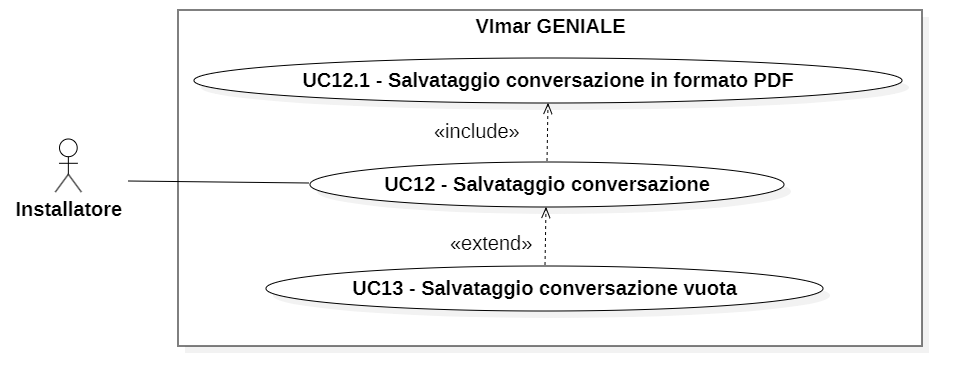
\includegraphics[width=1\textwidth]{contents/casi_duso/png/UC12.png}
\caption{UC12 - Salvataggio conversazione}
% \label{fig:UC1a}
\end{figure}

\subuc{Salvataggio conversazione in formato PDF}{salvataggio_conv_PDF}
\begin{itemize}
    \item \textbf{Attori coinvolti}: Installatore;
    \item \textbf{Descrizione}: L’installatore, prima di chiudere l’applicativo, desidera salvare in formato PDF una conversazione memorizzata attualmente all’interno del \textit{sistema}\textsubscript{G}, per poterla consultare dopo aver chiuso l'applicativo;
    \item \textbf{Precondizioni}: 
    \begin{itemize}
        \item L’installatore ha accesso all’\textit{interfaccia web}\textsubscript{G} del \textit{sistema}\textsubscript{G};
        \item L’installatore ha accesso ad una conversazione memorizzabile nel \textit{sistema}\textsubscript{G}.
    \end{itemize}
    \item \textbf{Postcondizioni}: Il \textit{sistema}\textsubscript{G} salva in formato PDF la conversazione selezionata e memorizzata attualmente all’interno del \textit{sistema}\textsubscript{G};
    \item \textbf{Scenario principale}:
    \begin{enumerate}
        \item L’installatore accede all’\textit{interfaccia web}\textsubscript{G} di Vimar GENIALE;
        \item Richiede il salvataggio in formato PDF di una conversazione memorizzata attualmente all'interno del sistema;
        \item Il \textit{sistema}\textsubscript{G} effettua il salvataggio in formato PDF e fornisce una risposta che conferma il completamento dell’operazione;
        \item L’installatore visualizza il messaggio di conferma dell’avvenuto salvataggio.
    \end{enumerate}
\end{itemize}

\uc{Salvataggio conversazione vuota}{assenza_conv}
\begin{itemize}
    \item \textbf{Attori coinvolti}: Installatore;
    \item \textbf{Descrizione}: L’installatore tenta di salvare una conversazione vuota;
    \item \textbf{Precondizioni}: 
    \begin{itemize}
        \item L’installatore ha accesso all’\textit{interfaccia web}\textsubscript{G} del \textit{sistema}\textsubscript{G};
        \item L'installatore crea una nuova \textit{conversazione libera}\textsubscript{G} e poi non fa nessuna domanda.
    \end{itemize}
    \item \textbf{Postcondizioni}: Il \textit{sistema}\textsubscript{G} restituisce una risposta che indica il motivo per cui si è verificato l’errore;
    \item \textbf{Scenario principale}:
    \begin{enumerate}
        \item L’installatore accede all’\textit{interfaccia web}\textsubscript{G} di Vimar GENIALE;
        \item L'installatore crea una nuova conversazione, ma non pone nessuna domanda;
        \item Richiede il salvataggio della conversazione appena creata;
        \item Il \textit{sistema}\textsubscript{G} elabora la richiesta e fornisce una risposta che spiega la causa dell'errore riscontrato;
        \item L’installatore visualizza le informazioni sull’errore che si è verificato.
    \end{enumerate}
\end{itemize}



\uc{Accesso al \textit{cruscotto informativo}\textsubscript{G}}{accesso_cruscotto}
\begin{itemize}
    \item \textbf{Attori coinvolti}: \textit{Amministratore}\textsubscript{G};
    \item \textbf{Descrizione}: Un \textit{amministratore}\textsubscript{G} desidera accedere al \textit{cruscotto informativo}\textsubscript{G} per visualizzare una panoramica di informazioni relative all’utilizzo del \textit{sistema}\textsubscript{G};
    \item \textbf{Precondizioni}: 
    \begin{itemize}
        \item L’\textit{amministratore}\textsubscript{G} ha accesso all’\textit{interfaccia web}\textsubscript{G} del \textit{sistema}\textsubscript{G};
        \item L’\textit{amministratore}\textsubscript{G} è dotato delle credenziali necessarie ad accedere alla \textit{dashboard}\textsubscript{G}.
    \end{itemize}
    \item \textbf{Postcondizioni}: L’\textit{amministratore}\textsubscript{G} accede al \textit{cruscotto informativo}\textsubscript{G}, da cui può visualizzare svariate informazioni riguardanti l’uso del \textit{sistema}\textsubscript{G};
    \item \textbf{Scenario principale}:
    \begin{enumerate}
        \item L’\textit{amministratore}\textsubscript{G} accede all’\textit{interfaccia web}\textsubscript{G} di Vimar GENIALE;
        \item Inserisce le proprie credenziali;
        \item Il \textit{sistema}\textsubscript{G} riceve la richiesta di accesso e \textit{verifica}\textsubscript{G} le credenziali;
        \item L’\textit{amministratore}\textsubscript{G} ottiene l’accesso alla \textit{dashboard}\textsubscript{G}.
    \end{enumerate}
    \item \textbf{Inclusioni}: UC14.1 - Inserimento \textit{username}\textsubscript{G} e \textit{password}\textsubscript{G};
    \item \textbf{Estensioni}: UC15 - Inserimento \textit{username}\textsubscript{G} o \textit{password}\textsubscript{G} errati.
\end{itemize}
\begin{figure}[H]
\centering
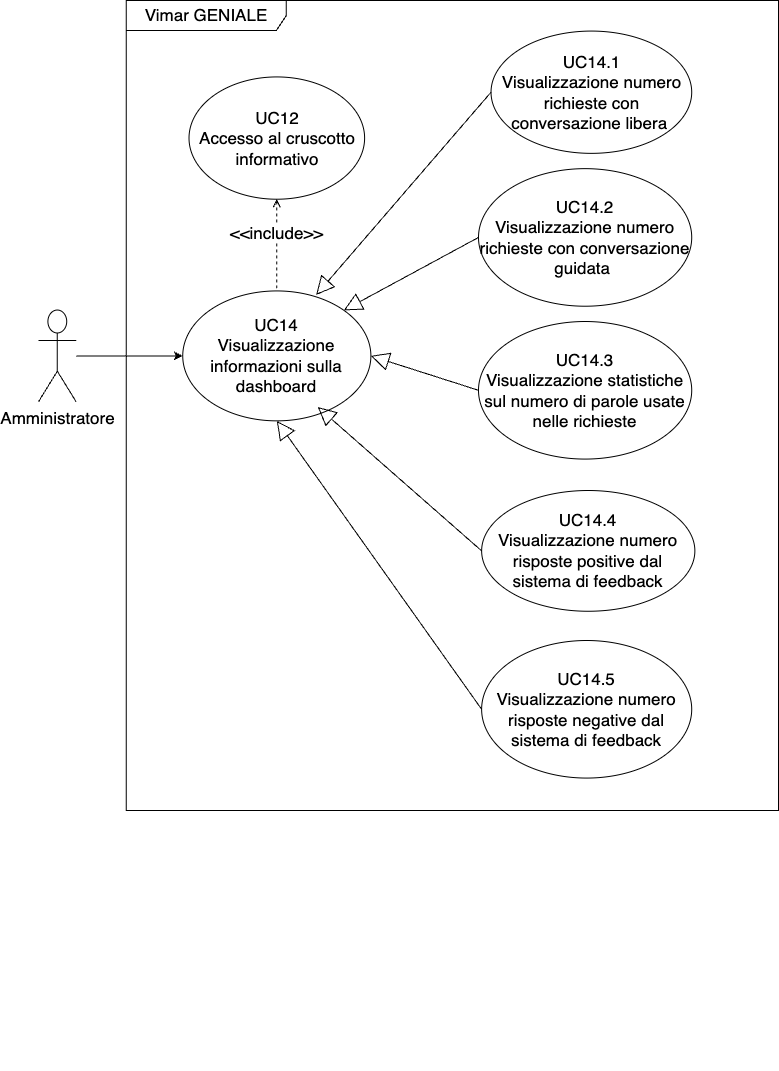
\includegraphics[width=1\textwidth]{contents/casi_duso/png/UC14.png}
\caption{UC14 - Accesso al \textit{cruscotto informativo}\textsubscript{G}}
% \label{fig:UC1a}
\end{figure}

\subuc{Inserimento \textit{username}\textsubscript{G} e \textit{password}\textsubscript{G}}{inserimento_cred}
\begin{itemize}
    \item \textbf{Attori coinvolti}: \textit{Amministratore}\textsubscript{G};
    \item \textbf{Descrizione}: Un \textit{amministratore}\textsubscript{G} desidera accedere al \textit{cruscotto informativo}\textsubscript{G} per visualizzare una panoramica di informazioni relative all’utilizzo del \textit{sistema}\textsubscript{G}, dunque inserisce lo \textit{username}\textsubscript{G} e la \textit{password}\textsubscript{G};
    \item \textbf{Precondizioni}: 
    \begin{itemize}
        \item L’\textit{amministratore}\textsubscript{G} ha accesso all’\textit{interfaccia web}\textsubscript{G} del \textit{sistema}\textsubscript{G};
        \item L’\textit{amministratore}\textsubscript{G} è dotato dello \textit{username}\textsubscript{G} e della \textit{password}\textsubscript{G} necessarie ad accedere alla \textit{dashboard}\textsubscript{G}.
    \end{itemize}
    \item \textbf{Postcondizioni}: L’\textit{amministratore}\textsubscript{G} ha inserito lo \textit{username}\textsubscript{G} e la \textit{password}\textsubscript{G}, ovvero le credenziali richieste per l’accesso al \textit{cruscotto informativo}\textsubscript{G};
    \item \textbf{Scenario principale}:
    \begin{enumerate}
        \item L’\textit{amministratore}\textsubscript{G} accede all’\textit{interfaccia web}\textsubscript{G} di Vimar GENIALE;
        \item Inserisce lo \textit{username}\textsubscript{G};
        \item Inserisce la \textit{password}\textsubscript{G}.
    \end{enumerate}
\end{itemize}

\uc{Inserimento \textit{username}\textsubscript{G} o \textit{password}\textsubscript{G} errati}{inserimento_cred_errati}
\begin{itemize}
    \item \textbf{Attori coinvolti}: \textit{Amministratore}\textsubscript{G};
    \item \textbf{Descrizione}: Un \textit{amministratore}\textsubscript{G} desidera accedere al \textit{cruscotto informativo}\textsubscript{G} per visualizzare una panoramica di informazioni relative all’utilizzo del \textit{sistema}\textsubscript{G}, ma non riesce ad accedere a causa di un errore nell’inserimento dello \textit{username}\textsubscript{G} o della \textit{password}\textsubscript{G};
    \item \textbf{Precondizioni}: 
    \begin{itemize}
        \item L’\textit{amministratore}\textsubscript{G} ha accesso all’\textit{interfaccia web}\textsubscript{G} del \textit{sistema}\textsubscript{G};
        \item L’\textit{amministratore}\textsubscript{G} è dotato delle credenziali necessarie ad accedere alla \textit{dashboard}\textsubscript{G};
        \item Lo \textit{username}\textsubscript{G} o la \textit{password}\textsubscript{G} non sono corretti.
    \end{itemize}
    \item \textbf{Postcondizioni}: Il \textit{sistema}\textsubscript{G} restituisce una risposta che indica il motivo per cui si è verificato l’errore;
    \item \textbf{Scenario principale}:
    \begin{enumerate}
        \item L’\textit{amministratore}\textsubscript{G} accede all’\textit{interfaccia web}\textsubscript{G} di Vimar GENIALE;
        \item Inserisce le proprie credenziali;
        \item Il \textit{sistema}\textsubscript{G} elabora la richiesta e fornisce una risposta che spiega l’inserimento errato delle credenziali;
        \item L’\textit{amministratore}\textsubscript{G} visualizza le informazioni sull’errore che si è verificato.
    \end{enumerate}
\end{itemize}



\uc{Visualizzazione informazioni sulla \textit{dashboard}\textsubscript{G}}{visualizzazione_info_dashboard}
\begin{itemize}
    \item \textbf{Attori coinvolti}: \textit{Amministratore}\textsubscript{G};
    \item \textbf{Descrizione}: Un \textit{amministratore}\textsubscript{G} desidera visualizzare una panoramica di informazioni relative all’utilizzo del \textit{sistema}\textsubscript{G} dal \textit{cruscotto informativo}\textsubscript{G};
    \item \textbf{Precondizioni}: 
    \begin{itemize}
        \item L’\textit{amministratore}\textsubscript{G} ha accesso all’\textit{interfaccia web}\textsubscript{G} del \textit{sistema}\textsubscript{G};
        \item L’\textit{amministratore}\textsubscript{G} è dotato dell’accesso alla \textit{dashboard}\textsubscript{G}.
    \end{itemize}
    \item \textbf{Postcondizioni}: Il \textit{sistema}\textsubscript{G} raccoglie le informazioni richieste e le mostra nella \textit{dashboard}\textsubscript{G};
    \item \textbf{Scenario principale}:
    \begin{enumerate}
        \item L’\textit{amministratore}\textsubscript{G} accede all’\textit{interfaccia web}\textsubscript{G} di Vimar GENIALE;
        \item Inserisce le proprie credenziali;
        \item Il \textit{sistema}\textsubscript{G} riceve la richiesta di accesso e \textit{verifica}\textsubscript{G} le credenziali;
        \item L’\textit{amministratore}\textsubscript{G} ottiene l’accesso alla \textit{dashboard}\textsubscript{G};
        \item Il \textit{sistema}\textsubscript{G} mostra le informazioni richieste sul \textit{cruscotto informativo}\textsubscript{G}.
    \end{enumerate}
    \item \textbf{Inclusioni}: 
    \begin{itemize}
        \item UC16.1 - Visualizzazione numero richieste con \textit{conversazione libera}\textsubscript{G};
        \item UC16.2 - Visualizzazione numero richieste con \textit{conversazione guidata}\textsubscript{G};
        \item UC16.3 - Visualizzazione classifica di parole più utilizzate;
        \item UC16.4 - Visualizzazione numero risposte positive dal \textit{sistema}\textsubscript{G} di \textit{feedback}\textsubscript{G};
        \item UC16.5 - Visualizzazione numero negative positive dal \textit{sistema}\textsubscript{G} di \textit{feedback}\textsubscript{G}.
    \end{itemize}
\end{itemize}
\begin{figure}[H]
\centering
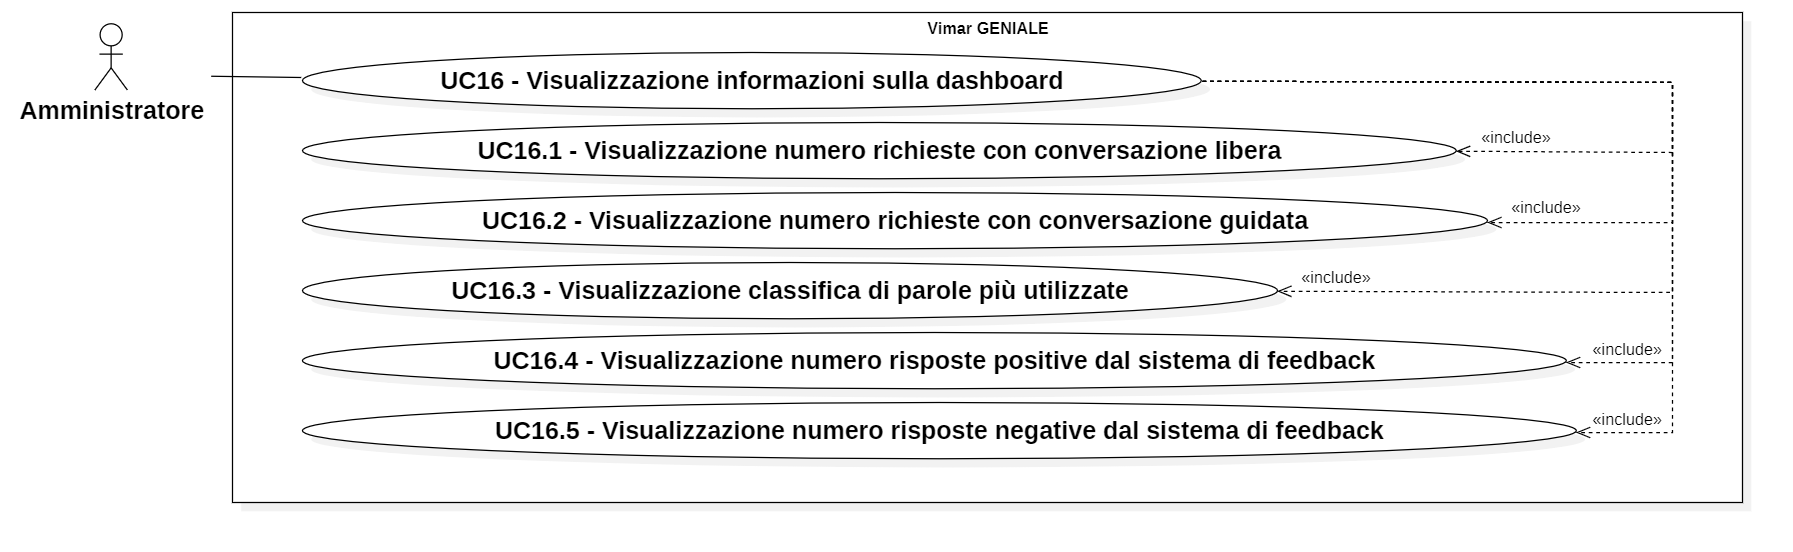
\includegraphics[width=1\textwidth]{contents/casi_duso/png/UC16.png}
\caption{UC16 - Visualizzazione informazioni sulla \textit{dashboard}\textsubscript{G}}
% \label{fig:UC1a}
\end{figure}

\subuc{Visualizzazione numero richieste con \textit{conversazione libera}\textsubscript{G}}{visualizzazione_richieste_libere}
\begin{itemize}
    \item \textbf{Attori coinvolti}: \textit{Amministratore}\textsubscript{G};
    \item \textbf{Descrizione}: Un \textit{amministratore}\textsubscript{G} desidera visualizzare dal \textit{cruscotto informativo}\textsubscript{G} il numero delle richieste effettuate con una \textit{conversazione libera}\textsubscript{G};
    \item \textbf{Precondizioni}: 
    \begin{itemize}
        \item L’\textit{amministratore}\textsubscript{G} ha accesso all’\textit{interfaccia web}\textsubscript{G} del \textit{sistema}\textsubscript{G};
        \item L’\textit{amministratore}\textsubscript{G} è dotato dell’accesso alla \textit{dashboard}\textsubscript{G}.
    \end{itemize}
    \item \textbf{Postcondizioni}: Il \textit{sistema}\textsubscript{G} raccoglie le informazioni relative al numero delle richieste effettuate con una \textit{conversazione libera}\textsubscript{G} e le mostra nella \textit{dashboard}\textsubscript{G};
    \item \textbf{Scenario principale}:
    \begin{enumerate}
        \item L’\textit{amministratore}\textsubscript{G} accede all’\textit{interfaccia web}\textsubscript{G} di Vimar GENIALE;
        \item Inserisce le proprie credenziali;
        \item Il \textit{sistema}\textsubscript{G} riceve la richiesta di accesso e \textit{verifica}\textsubscript{G} le credenziali;
        \item L’\textit{amministratore}\textsubscript{G} ottiene l’accesso alla \textit{dashboard}\textsubscript{G};
        \item Il \textit{sistema}\textsubscript{G} mostra le informazioni richieste sul \textit{cruscotto informativo}\textsubscript{G}.
    \end{enumerate}
\end{itemize}

\subuc{Visualizzazione numero richieste con \textit{conversazione guidata}\textsubscript{G}}{visualizzazione_richieste_guidate}
\begin{itemize}
    \item \textbf{Attori coinvolti}: \textit{Amministratore}\textsubscript{G};
    \item \textbf{Descrizione}: Un \textit{amministratore}\textsubscript{G} desidera visualizzare dal \textit{cruscotto informativo}\textsubscript{G} il numero delle richieste effettuate con una \textit{conversazione guidata}\textsubscript{G};
    \item \textbf{Precondizioni}: 
    \begin{itemize}
        \item L’\textit{amministratore}\textsubscript{G} ha accesso all’\textit{interfaccia web}\textsubscript{G} del \textit{sistema}\textsubscript{G};
        \item L’\textit{amministratore}\textsubscript{G} è dotato dell’accesso alla \textit{dashboard}\textsubscript{G}.
    \end{itemize}
    \item \textbf{Postcondizioni}: Il \textit{sistema}\textsubscript{G} raccoglie le informazioni relative al numero delle richieste effettuate con una \textit{conversazione guidata}\textsubscript{G} e le mostra nella \textit{dashboard}\textsubscript{G};
    \item \textbf{Scenario principale}:
    \begin{enumerate}
        \item L’\textit{amministratore}\textsubscript{G} accede all’\textit{interfaccia web}\textsubscript{G} di Vimar GENIALE;
        \item Inserisce le proprie credenziali;
        \item Il \textit{sistema}\textsubscript{G} riceve la richiesta di accesso e \textit{verifica}\textsubscript{G} le credenziali;
        \item L’\textit{amministratore}\textsubscript{G} ottiene l’accesso alla \textit{dashboard}\textsubscript{G};
        \item Il \textit{sistema}\textsubscript{G} mostra le informazioni richieste sul \textit{cruscotto informativo}\textsubscript{G}.
    \end{enumerate}
\end{itemize}

\subuc{Visualizzazione classifica di parole più utilizzate}{visualizzazione_statistiche_parole}
\begin{itemize}
    \item \textbf{Attori coinvolti}: \textit{Amministratore}\textsubscript{G};
    \item \textbf{Descrizione}: Un \textit{amministratore}\textsubscript{G} desidera visualizzare dal \textit{cruscotto informativo}\textsubscript{G} la classifica delle parole più utilizzate con relativa percentuale rispetto al numero totale delle parole utilizzate nelle richieste;
    \item \textbf{Precondizioni}: 
    \begin{itemize}
        \item L’\textit{amministratore}\textsubscript{G} ha accesso all’\textit{interfaccia web}\textsubscript{G} del \textit{sistema}\textsubscript{G};
        \item L’\textit{amministratore}\textsubscript{G} è dotato dell’accesso alla \textit{dashboard}\textsubscript{G}.
    \end{itemize}
    \item \textbf{Postcondizioni}: Il \textit{sistema}\textsubscript{G} raccoglie le informazioni relative alla classifica delle parole più utilizzate nelle richieste e la mostra nella \textit{dashboard}\textsubscript{G};
    \item \textbf{Scenario principale}:
    \begin{enumerate}
        \item L’\textit{amministratore}\textsubscript{G} accede all’\textit{interfaccia web}\textsubscript{G} di Vimar GENIALE;
        \item Inserisce le proprie credenziali;
        \item Il \textit{sistema}\textsubscript{G} riceve la richiesta di accesso e \textit{verifica}\textsubscript{G} le credenziali;
        \item L’\textit{amministratore}\textsubscript{G} ottiene l’accesso alla \textit{dashboard}\textsubscript{G};
        \item Il \textit{sistema}\textsubscript{G} mostra le informazioni richieste sul \textit{cruscotto informativo}\textsubscript{G}.
    \end{enumerate}
\end{itemize}

\subuc{Visualizzazione numero risposte positive dal \textit{sistema}\textsubscript{G} di \textit{feedback}\textsubscript{G}}{visualizzazione_risposte_positive}
\begin{itemize}
    \item \textbf{Attori coinvolti}: \textit{Amministratore}\textsubscript{G};
    \item \textbf{Descrizione}: Un \textit{amministratore}\textsubscript{G} desidera visualizzare dal \textit{cruscotto informativo}\textsubscript{G} il numero delle risposte positive dal \textit{sistema}\textsubscript{G} di \textit{feedback}\textsubscript{G};
    \item \textbf{Precondizioni}: 
    \begin{itemize}
        \item L’\textit{amministratore}\textsubscript{G} ha accesso all’\textit{interfaccia web}\textsubscript{G} del \textit{sistema}\textsubscript{G};
        \item L’\textit{amministratore}\textsubscript{G} è dotato dell’accesso alla \textit{dashboard}\textsubscript{G}.
    \end{itemize}
    \item \textbf{Postcondizioni}: Il \textit{sistema}\textsubscript{G} raccoglie le informazioni relative al numero delle risposte positive dal \textit{sistema}\textsubscript{G} di \textit{feedback}\textsubscript{G} e le mostra nella \textit{dashboard}\textsubscript{G};
    \item \textbf{Scenario principale}:
    \begin{enumerate}
        \item L’\textit{amministratore}\textsubscript{G} accede all’\textit{interfaccia web}\textsubscript{G} di Vimar GENIALE;
        \item Inserisce le proprie credenziali;
        \item Il \textit{sistema}\textsubscript{G} riceve la richiesta di accesso e \textit{verifica}\textsubscript{G} le credenziali;
        \item L’\textit{amministratore}\textsubscript{G} ottiene l’accesso alla \textit{dashboard}\textsubscript{G};
        \item Il \textit{sistema}\textsubscript{G} mostra le informazioni richieste sul \textit{cruscotto informativo}\textsubscript{G}.
    \end{enumerate}
\end{itemize}

\subuc{Visualizzazione numero risposte negative dal \textit{sistema}\textsubscript{G} di \textit{feedback}\textsubscript{G}}{visualizzazione_risposte_negative}
\begin{itemize}
    \item \textbf{Attori coinvolti}: \textit{Amministratore}\textsubscript{G};
    \item \textbf{Descrizione}: Un \textit{amministratore}\textsubscript{G} desidera visualizzare dal \textit{cruscotto informativo}\textsubscript{G} il numero delle risposte negative dal \textit{sistema}\textsubscript{G} di \textit{feedback}\textsubscript{G};
    \item \textbf{Precondizioni}: 
    \begin{itemize}
        \item L’\textit{amministratore}\textsubscript{G} ha accesso all’\textit{interfaccia web}\textsubscript{G} del \textit{sistema}\textsubscript{G};
        \item L’\textit{amministratore}\textsubscript{G} è dotato dell’accesso alla \textit{dashboard}\textsubscript{G}.
    \end{itemize}
    \item \textbf{Postcondizioni}: Il \textit{sistema}\textsubscript{G} raccoglie le informazioni relative al numero delle risposte negative dal \textit{sistema}\textsubscript{G} di \textit{feedback}\textsubscript{G} e le mostra nella \textit{dashboard}\textsubscript{G};
    \item \textbf{Scenario principale}:
    \begin{enumerate}
        \item L’\textit{amministratore}\textsubscript{G} accede all’\textit{interfaccia web}\textsubscript{G} di Vimar GENIALE;
        \item Inserisce le proprie credenziali;
        \item Il \textit{sistema}\textsubscript{G} riceve la richiesta di accesso e \textit{verifica}\textsubscript{G} le credenziali;
        \item L’\textit{amministratore}\textsubscript{G} ottiene l’accesso alla \textit{dashboard}\textsubscript{G};
        \item Il \textit{sistema}\textsubscript{G} mostra le informazioni richieste sul \textit{cruscotto informativo}\textsubscript{G}.
    \end{enumerate}
\end{itemize}



\uc{Visualizzazione lista conversazioni}{visual_list_conv}
\begin{itemize}
    \item \textbf{Attori coinvolti}: Installatore;
    \item \textbf{Descrizione}: L'installatore vuole visualizzare la lista di tutte le conversazioni memorizzabili nel \textit{sistema}\textsubscript{G};
    \item \textbf{Precondizioni}: L’installatore ha accesso all’\textit{interfaccia web}\textsubscript{G} del \textit{sistema}\textsubscript{G};
    \item \textbf{Postcondizioni}: L'installatore visualizza la lista delle conversazioni presenti attualmente nell'applicativo;
    \item \textbf{Scenario principale}:
    \begin{enumerate}
        \item L’installatore ha accesso all’\textit{interfaccia web}\textsubscript{G} del \textit{sistema}\textsubscript{G};
        \item L'installatore visualizza la lista delle conversazioni presenti attualmente nel \textit{sistema}\textsubscript{G}.
    \end{enumerate}
    \item \textbf{Inclusioni}: UC17.1 - Visualizzazione singola conversazione.
\end{itemize}
\begin{figure}[H]
\centering
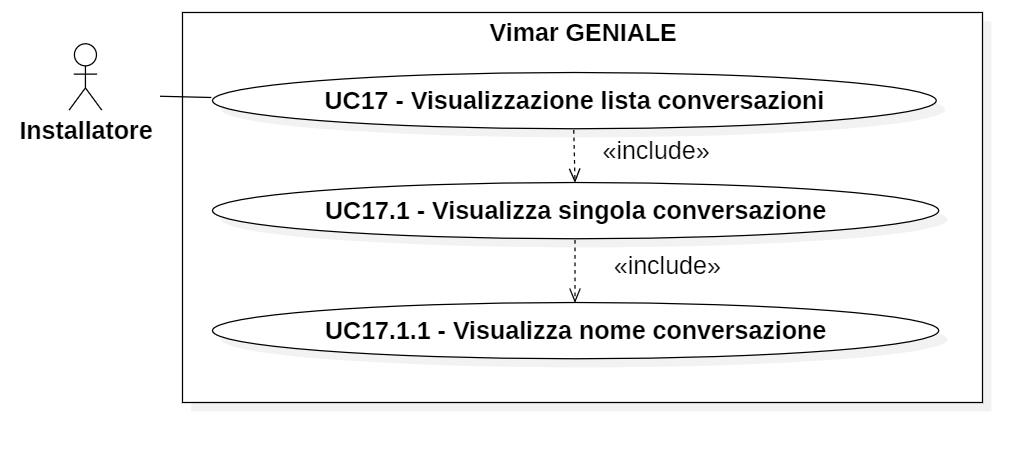
\includegraphics[width=1\textwidth]{contents/casi_duso/png/UC17.png}
\caption{UC17 - Visualizzazione lista conversazioni}
% \label{fig:UC1a}
\end{figure}

\subuc{Visualizzazione singola conversazione}{visual_conv}
\begin{itemize}
    \item \textbf{Attori coinvolti}: Installatore;
    \item \textbf{Descrizione}: L'installatore vuole visualizzare una singola conversazione;
    \item \textbf{Precondizioni}: L’installatore ha accesso all’\textit{interfaccia web}\textsubscript{G} del \textit{sistema}\textsubscript{G};
    \item \textbf{Postcondizioni}: L'installatore visualizza una singola conversazione;
    \item \textbf{Scenario principale}:
    \begin{enumerate}
        \item L’installatore ha accesso all’\textit{interfaccia web}\textsubscript{G} del \textit{sistema}\textsubscript{G};
        \item L'installatore visualizza una singola conversazione.
    \end{enumerate}
    \item \textbf{Inclusioni}: UC17.1.1 - Visualizzazione nome conversazione.
\end{itemize}

\subsubuc{Visualizzazione nome conversazione}{visual_nome_conv}
\begin{itemize}
    \item \textbf{Attori coinvolti}: Installatore;
    \item \textbf{Descrizione}: L'installatore vuole visualizzare il nome di una singola conversazione;
    \item \textbf{Precondizioni}: L’installatore ha accesso all’\textit{interfaccia web}\textsubscript{G} del \textit{sistema}\textsubscript{G};
    \item \textbf{Postcondizioni}: L'installatore visualizza il nome di una singola conversazione;
    \item \textbf{Scenario principale}:
    \begin{enumerate}
        \item L’installatore ha accesso all’\textit{interfaccia web}\textsubscript{G} del \textit{sistema}\textsubscript{G};
        \item L'installatore visualizza il nome di una singola conversazione.
    \end{enumerate}
\end{itemize}



\uc{Rinominazione della conversazione}{rinominazione_conv}
\begin{itemize}
    \item \textbf{Attori coinvolti}: Installatore;
    \item \textbf{Descrizione}: L'installatore vuole modificare il nome di una conversazione memorizzabile nel sistema;
    \item \textbf{Precondizioni}: L’installatore ha accesso all’\textit{interfaccia web}\textsubscript{G} del \textit{sistema}\textsubscript{G};
    \item \textbf{Postcondizioni}: L'installatore modifica il nome di una conversazione selezionata;
    \item \textbf{Scenario principale}:
    \begin{enumerate}
        \item L’installatore ha accesso all’\textit{interfaccia web}\textsubscript{G} del \textit{sistema}\textsubscript{G};
        \item L'installatore modifica il nome della conversazione selezionata.
    \end{enumerate}
\end{itemize}
\begin{figure}[H]
\centering
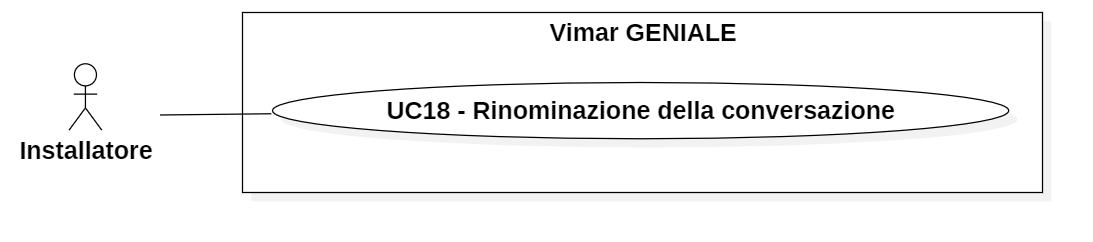
\includegraphics[width=1\textwidth]{contents/casi_duso/png/UC18.png}
\caption{UC18 - Rinominazione della conversazione}
% \label{fig:UC1a}
\end{figure}